\documentclass{beamer}
\usetheme{metropolis}
\usepackage{graphicx}
\usepackage{subfig}
\usepackage{tcolorbox}
\title{Computer Logic and Digital Circuit Design (PHYS306/COSC330): Week 1}
\author{Jordan Hanson}
\institute{Whittier College Department of Physics and Astronomy}

\begin{document}
\maketitle

\section{Summary}

\begin{frame}{Summary}
\begin{enumerate}
\item Logic functions
\begin{itemize}
\item Basic gate ideas
\item Combinatorial logic functions
\item Serial and parallel
\end{itemize}
\item Programmable logic (PL) vs. fixed integrated circuits (ICs)
\item Test instruments
\begin{itemize}
\item Oscilloscope
\item Signal generator
\item Digital voltmeter and DC power supply
\end{itemize}
\end{enumerate}
\end{frame}

\section{Analog Circuits}

\begin{frame}{Analog Circuits}
\small
First of all, what is an \textit{analog} circuit?
\begin{figure}
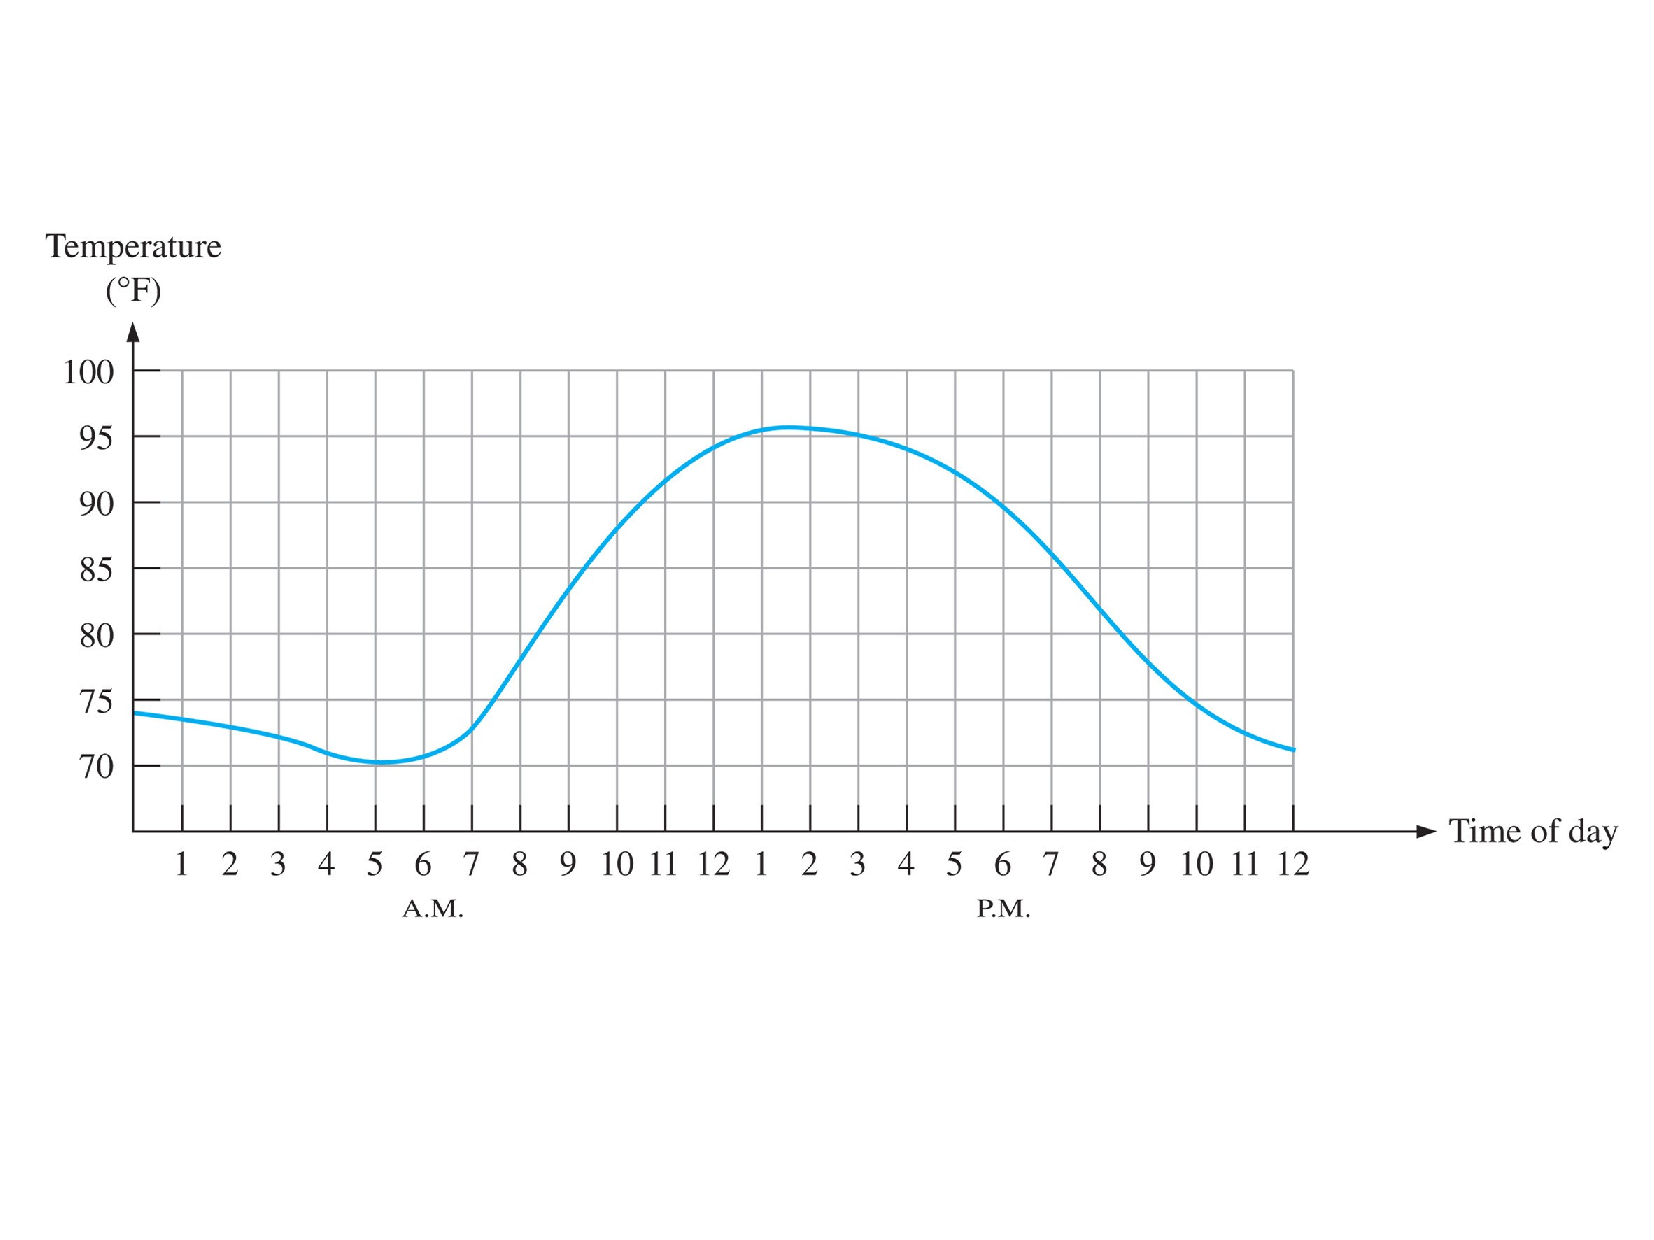
\includegraphics[width=0.8\textwidth,trim=0cm 4cm 0cm 4cm,clip=true]{analog1.pdf}
\caption{\label{fig:analog1} An example of an analog signal from a temperature sensor, converted from voltage.}
\end{figure}
\end{frame}

\begin{frame}{Analog Circuits}
\small
First of all, what is an \textit{analog} circuit?
\begin{figure}
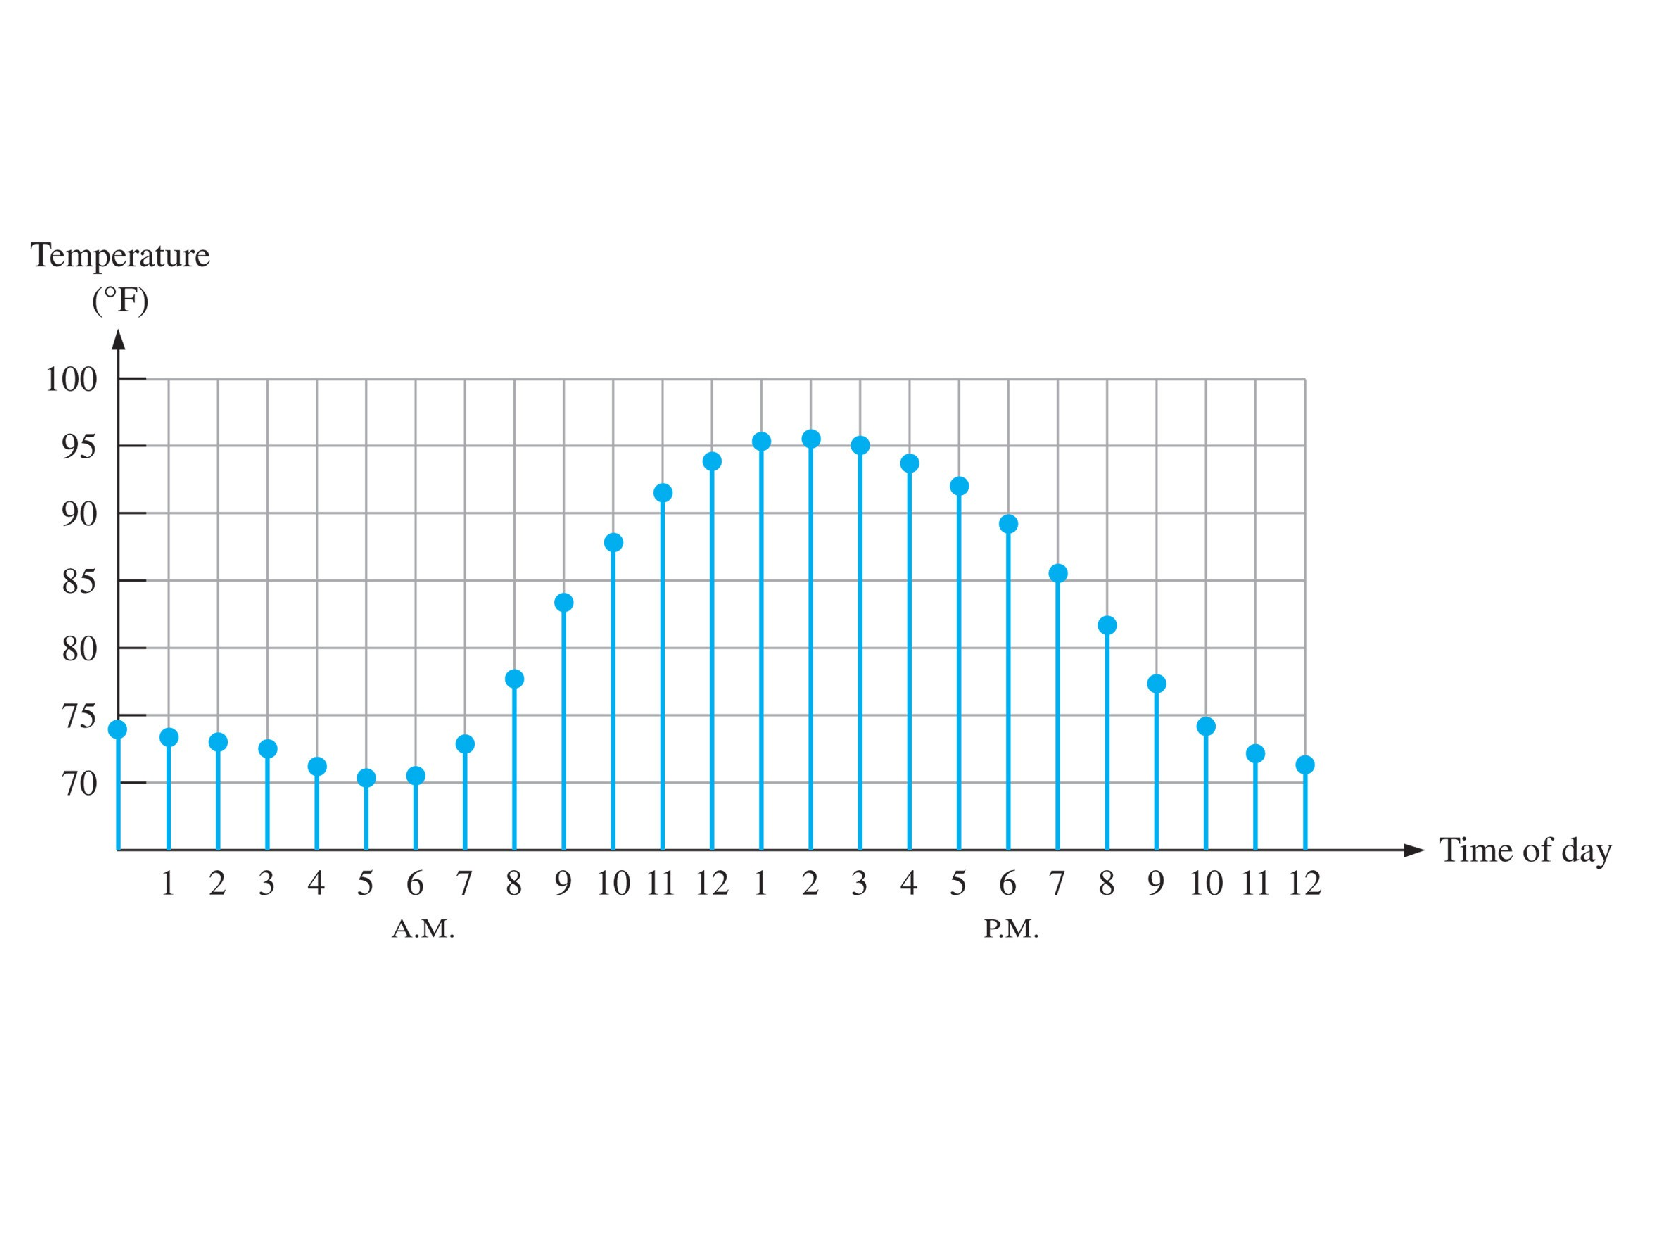
\includegraphics[width=0.8\textwidth,trim=0cm 4cm 0cm 4cm,clip=true]{analog2.pdf}
\caption{\label{fig:analog2} An example of that same signal, digitized and sampled.}
\end{figure}
Digital data forms the basis of computation:
\begin{itemize}
\item Noise issues, lossless transmission
\item Constructed from \textit{digits} ... 1 and 0
\end{itemize}
\end{frame}

\begin{frame}{Analog Circuits}
\small
First of all, what is an \textit{analog} circuit?
\begin{figure}
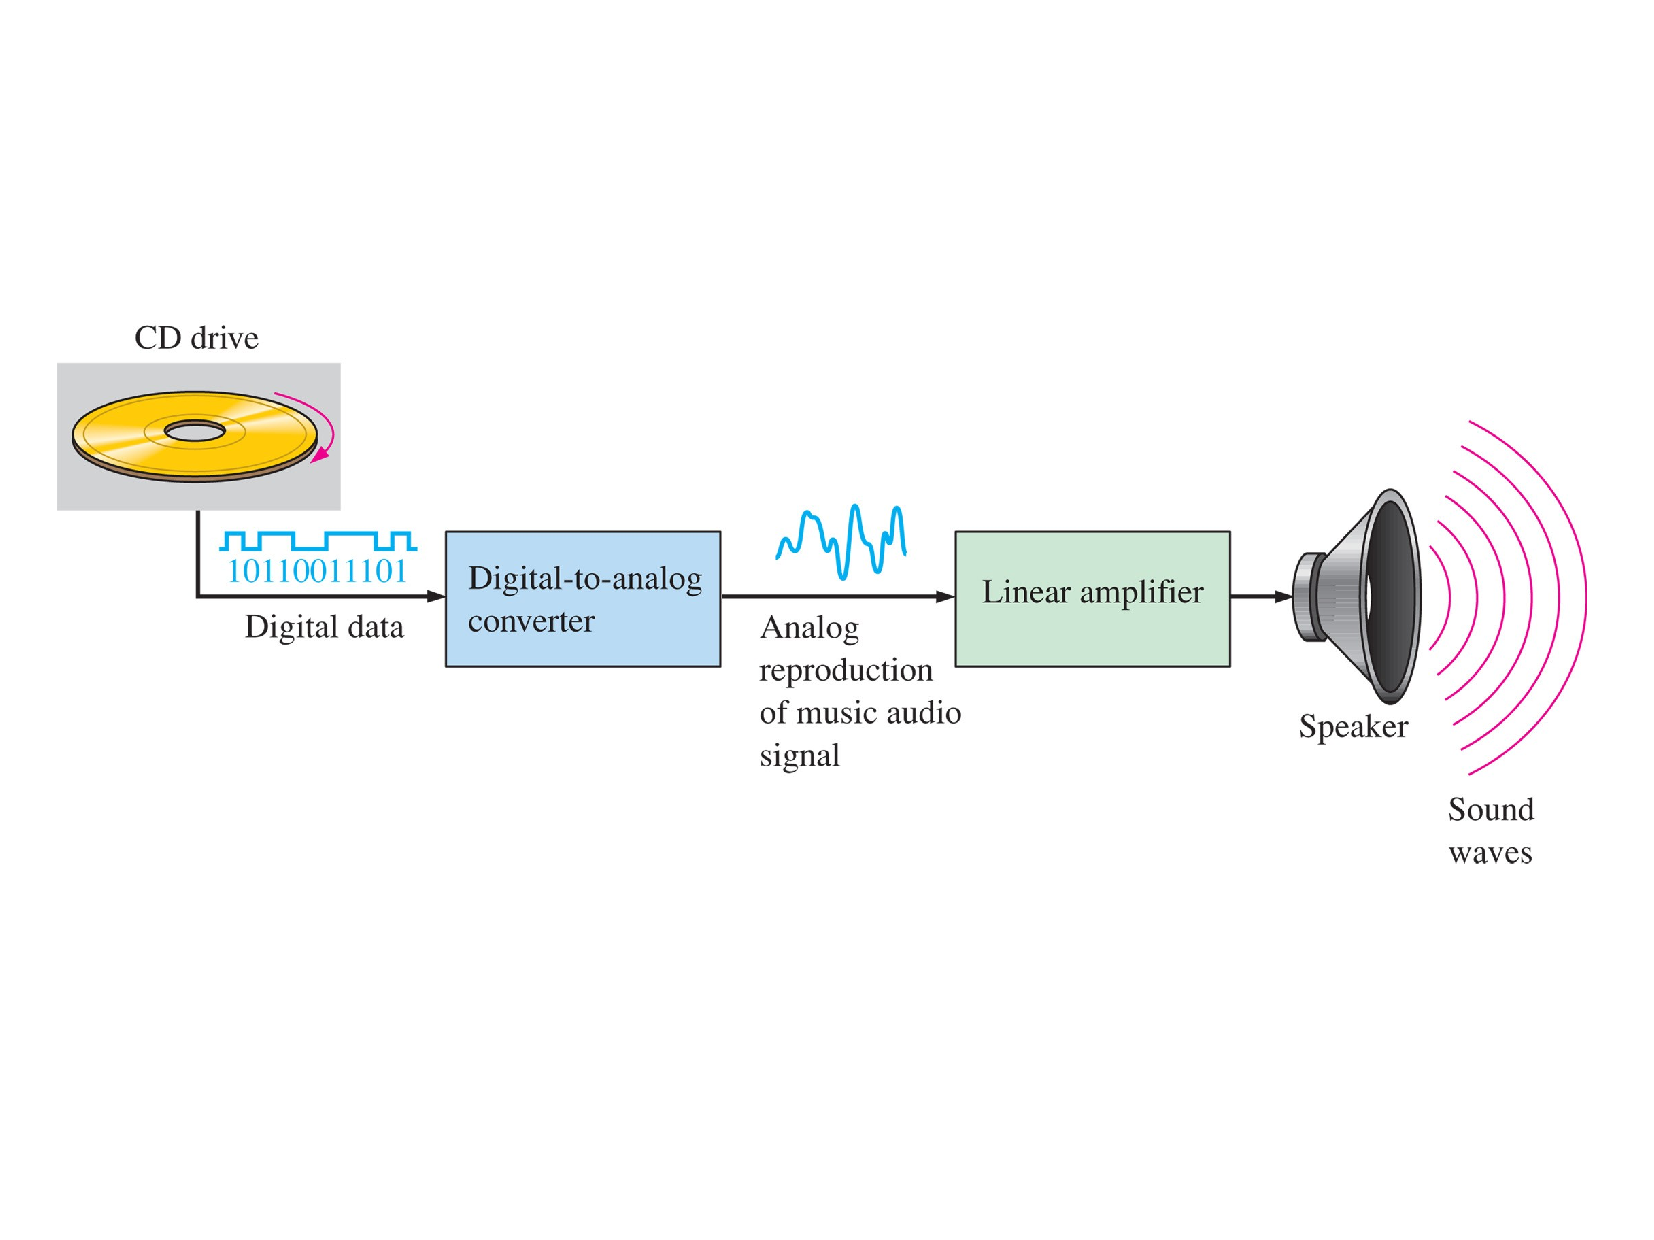
\includegraphics[width=0.8\textwidth,trim=0cm 4cm 0cm 4cm,clip=true]{analog3.pdf}
\caption{\label{fig:analog3} An example of a digital signal converted from binary to analog voltage signal.}
\end{figure}
\end{frame}

\begin{frame}{Analog Circuits}
One set of examples of analog circuits is RC/LC filters.  We must apply \textit{Ohm's Law} (Eq. \ref{eq:ohm}) and \textit{Kirchhoff's Rules} (Eqs. \ref{eq:kirchhoff1}-\ref{eq:kirchhoff2}) to understand these circuits, so let's review those.
\begin{align}
V &= IR \label{eq:ohm} \\
\sum_{i,node}^N j_i &= 0 \label{eq:kirchhoff1} \\
\sum_{i,loop}^N v_{i} &= 0 \label{eq:kirchhoff2}
\end{align}
\textbf{A node:} a point in a circuit where conductors meet.\\
\textbf{A loop:} a path in a circuit that returns to the same node.
\end{frame}

\begin{frame}{Analog Circuits}
\begin{figure}
\centering
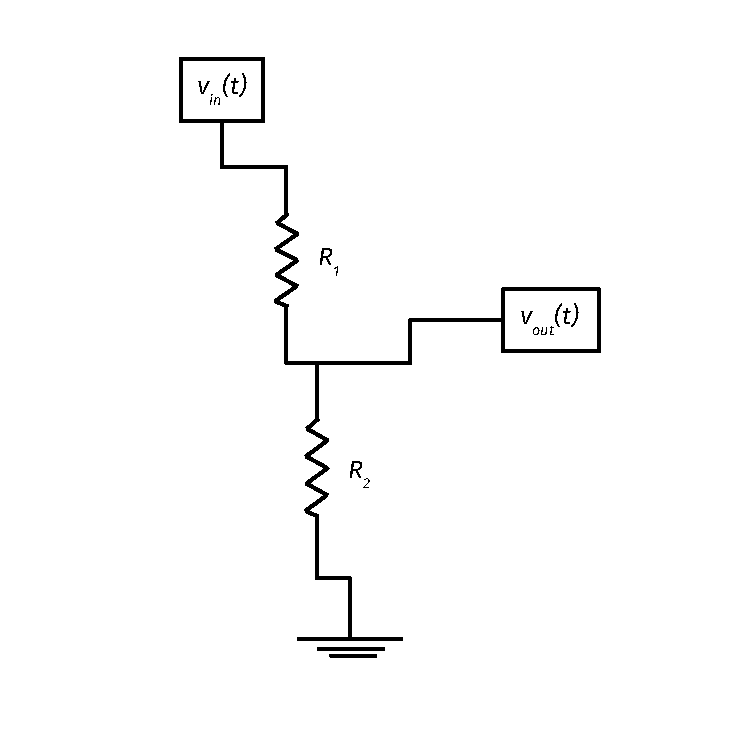
\includegraphics[width=0.5\textwidth]{VoltageDivider.pdf}
\caption{\label{fig:example1} A two-resistor voltage divider.}
\end{figure}
\end{frame}

\begin{frame}{Analog Circuits}
\begin{itemize}
\item Using Ohm's Law, find expressions for $v_{\rm in}(t)$ and $v_{\rm out}(t)$ in terms of the resistances and the current.
\item Take the ratio of the output voltage to the input voltage to find the \textbf{transfer function}, $H(t)$.
\end{itemize}
\end{frame}

\begin{frame}{Analog Circuits}
Answer:
\begin{equation}
H(t) = \frac{R_2}{R_1+R_2}
\end{equation}
Only the amplitude is affected:
\begin{itemize}
\item Original signal: $s_{in}(t) = A\cos(2\pi f t + \phi)$
\item New signal: $s_{out}(t) = A \left( \frac{R_1}{R_1+R_2}\right) \cos(2\pi f t + \phi)$
\end{itemize}
Other actions we can do in the time-domain:
\begin{itemize}
\item \textit{Delay}: shift the signal in time
\item \textit{Filter}: change which frequencies are most powerful
\item \textit{Integral/derivative}: circuit output is proportional to the integral or derivative of input
\end{itemize}
\end{frame}

\section{Logic Functions}

\begin{frame}{Logic Functions}
How do we build up digital data from analog signals?
\begin{figure}
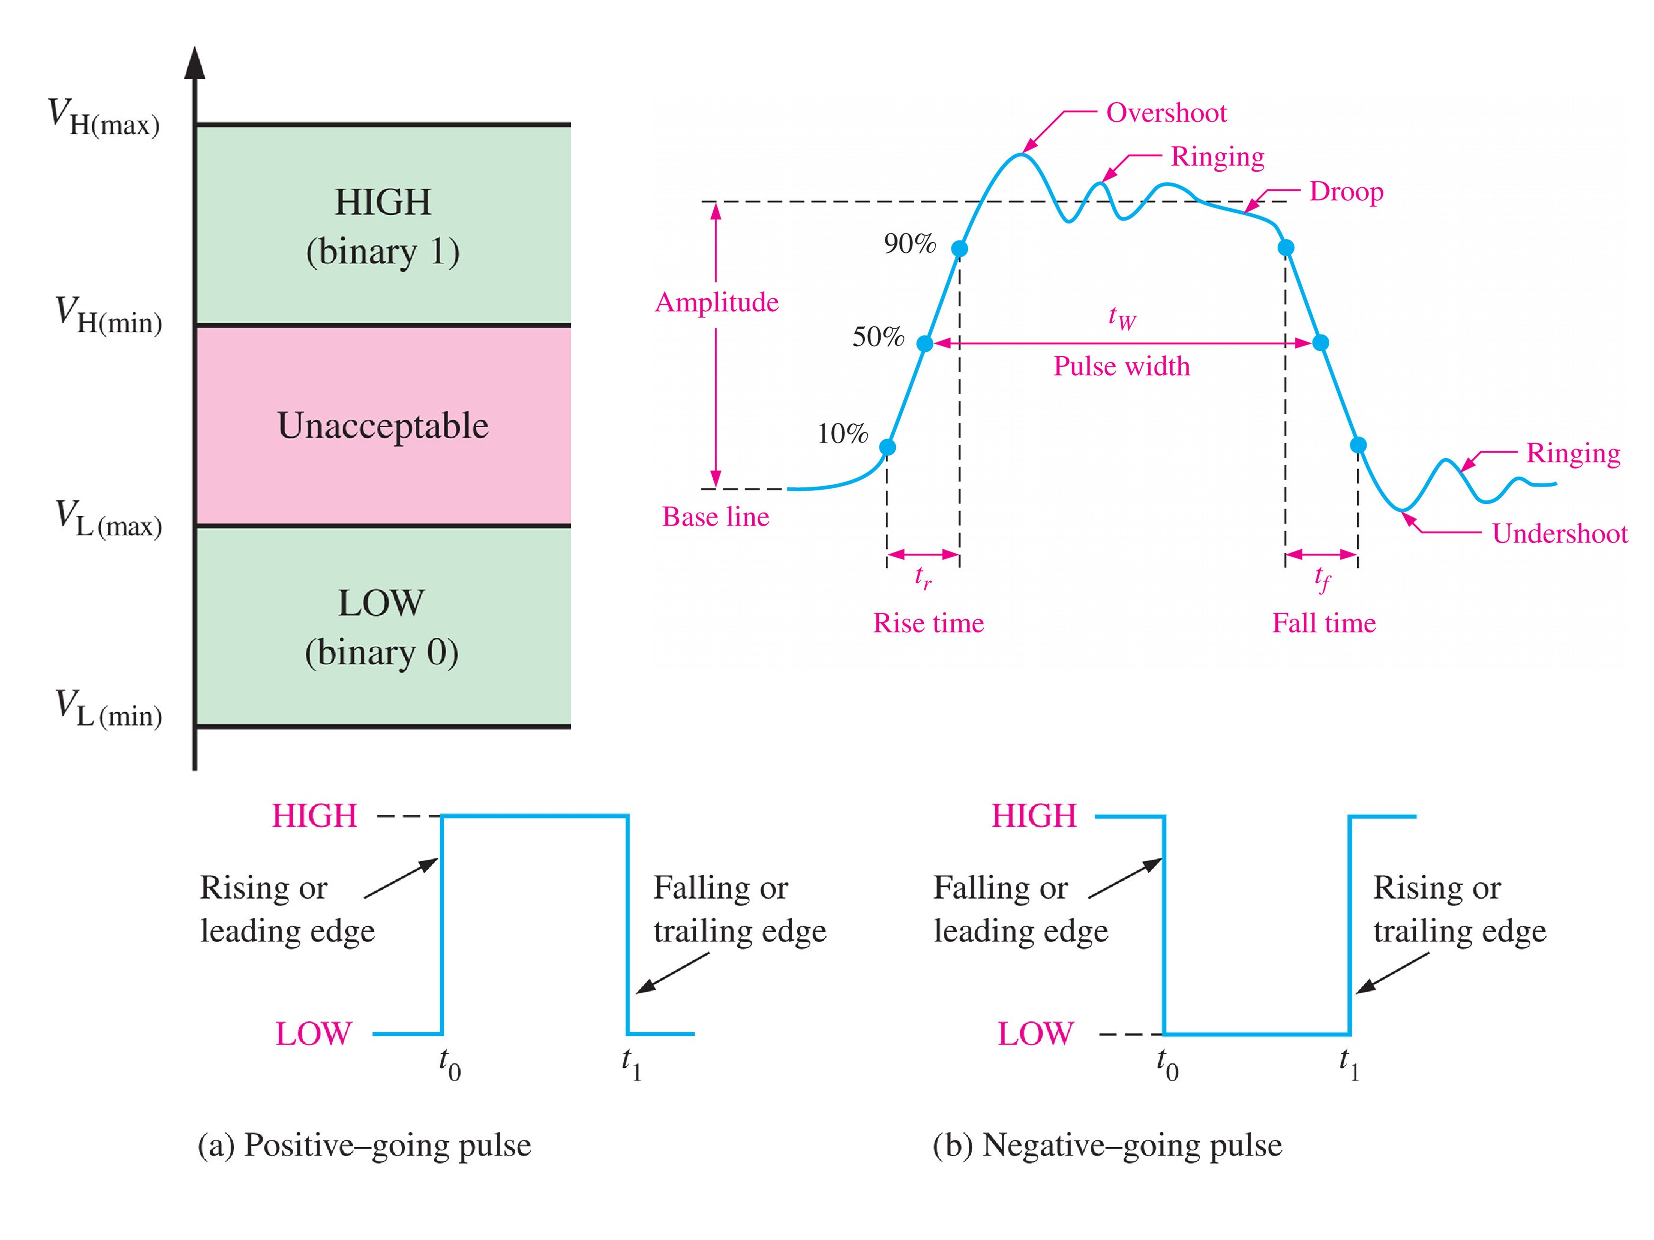
\includegraphics[width=0.75\textwidth]{digital1.pdf}
\caption{\label{fig:digital1} Logical ``1'' and ``0.''}
\end{figure}
\end{frame}

\begin{frame}{Logic Functions}
Terminology for digital signals:
\begin{enumerate}
\item \textbf{Frequency}, f and \textbf{period}, T: Signals per second, time between signals ($f = 1/T$).
\item \textbf{Pulse width}, $t_{\rm W}$: time duration a pulse is HIGH.
\item \textbf{Duty cycle}: $t_{\rm W}/T \times 100$\%
\end{enumerate}
\end{frame}

\begin{frame}{Logic Functions}
\begin{figure}
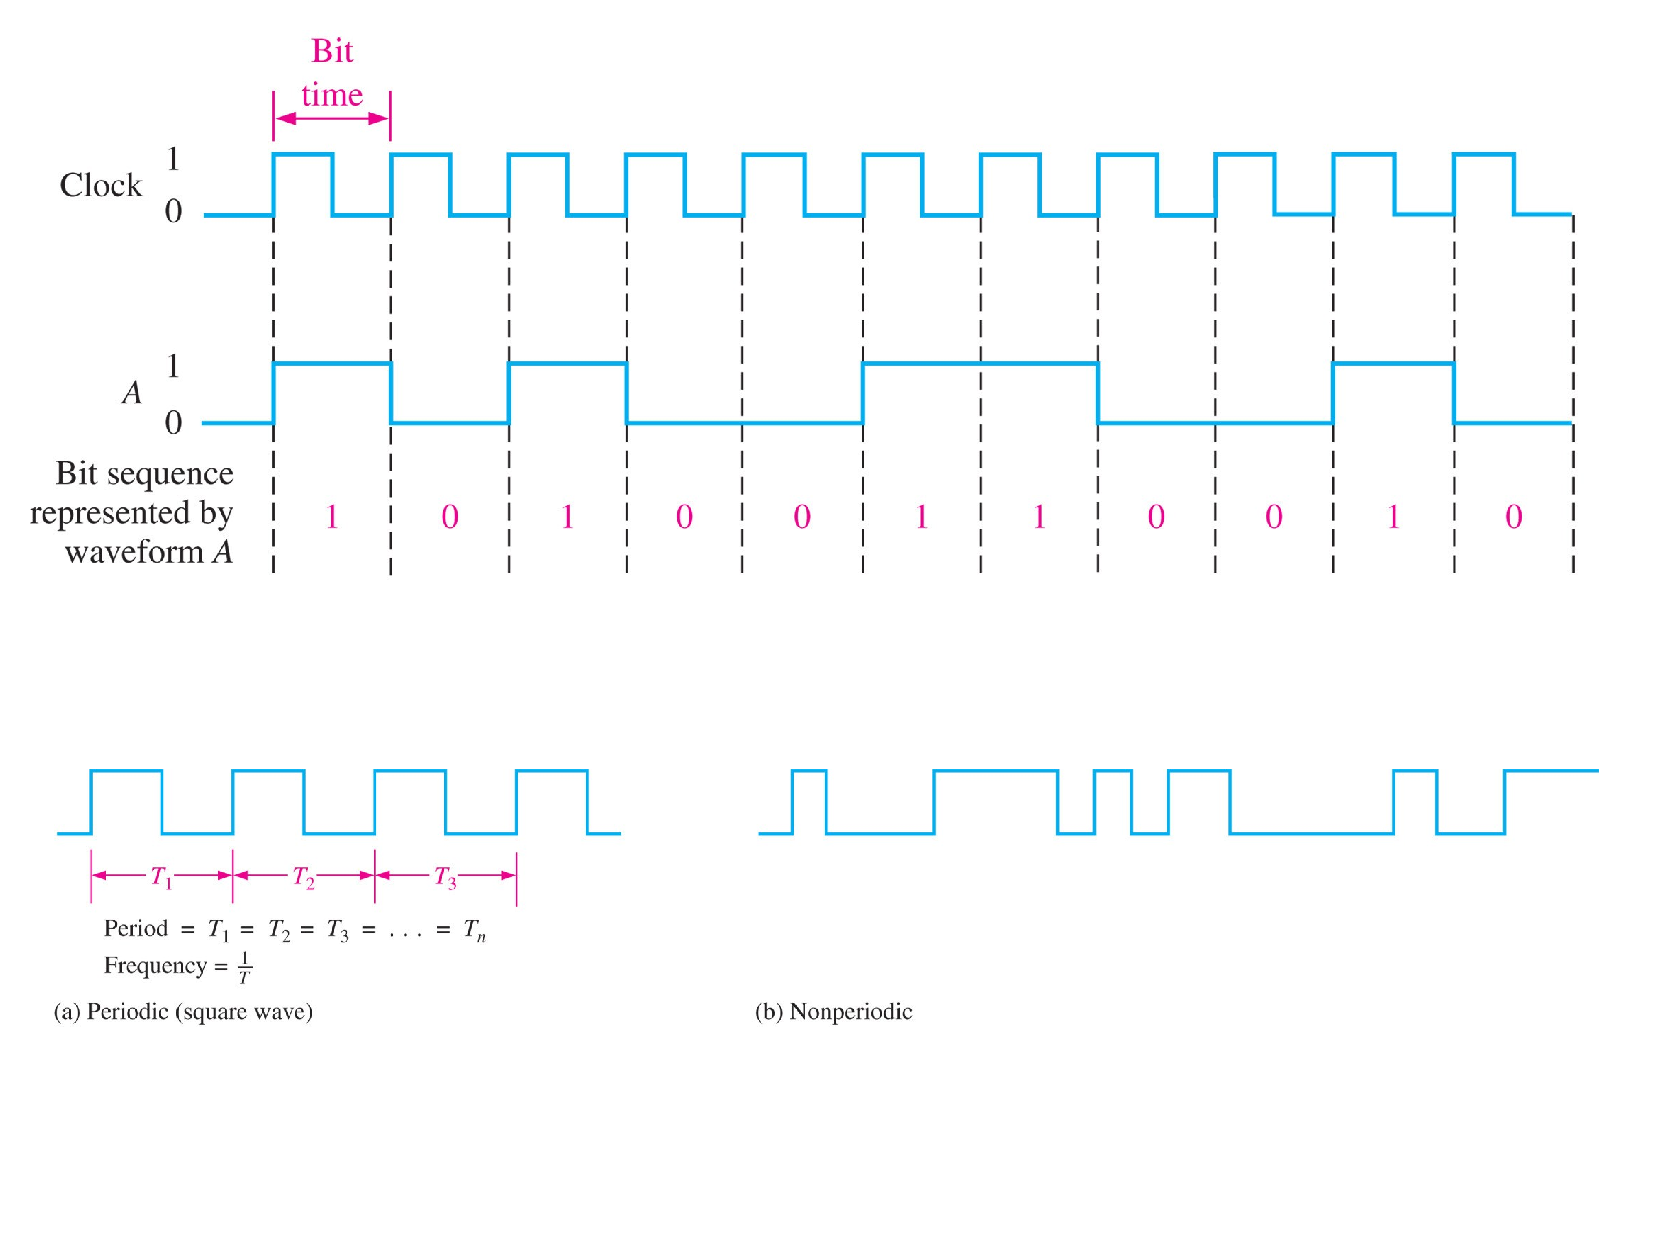
\includegraphics[width=0.75\textwidth]{digital2.pdf}
\caption{\label{fig:digital2} A clock signal is an example of a digital bitstream: alternating 1 and 0.  It has a period and a frequency.  Data can be \textit{periodic} or \textit{non-periodic}. (Professor: do some examples here).}
\end{figure}
\end{frame}

\begin{frame}{Logic Functions}
\begin{figure}
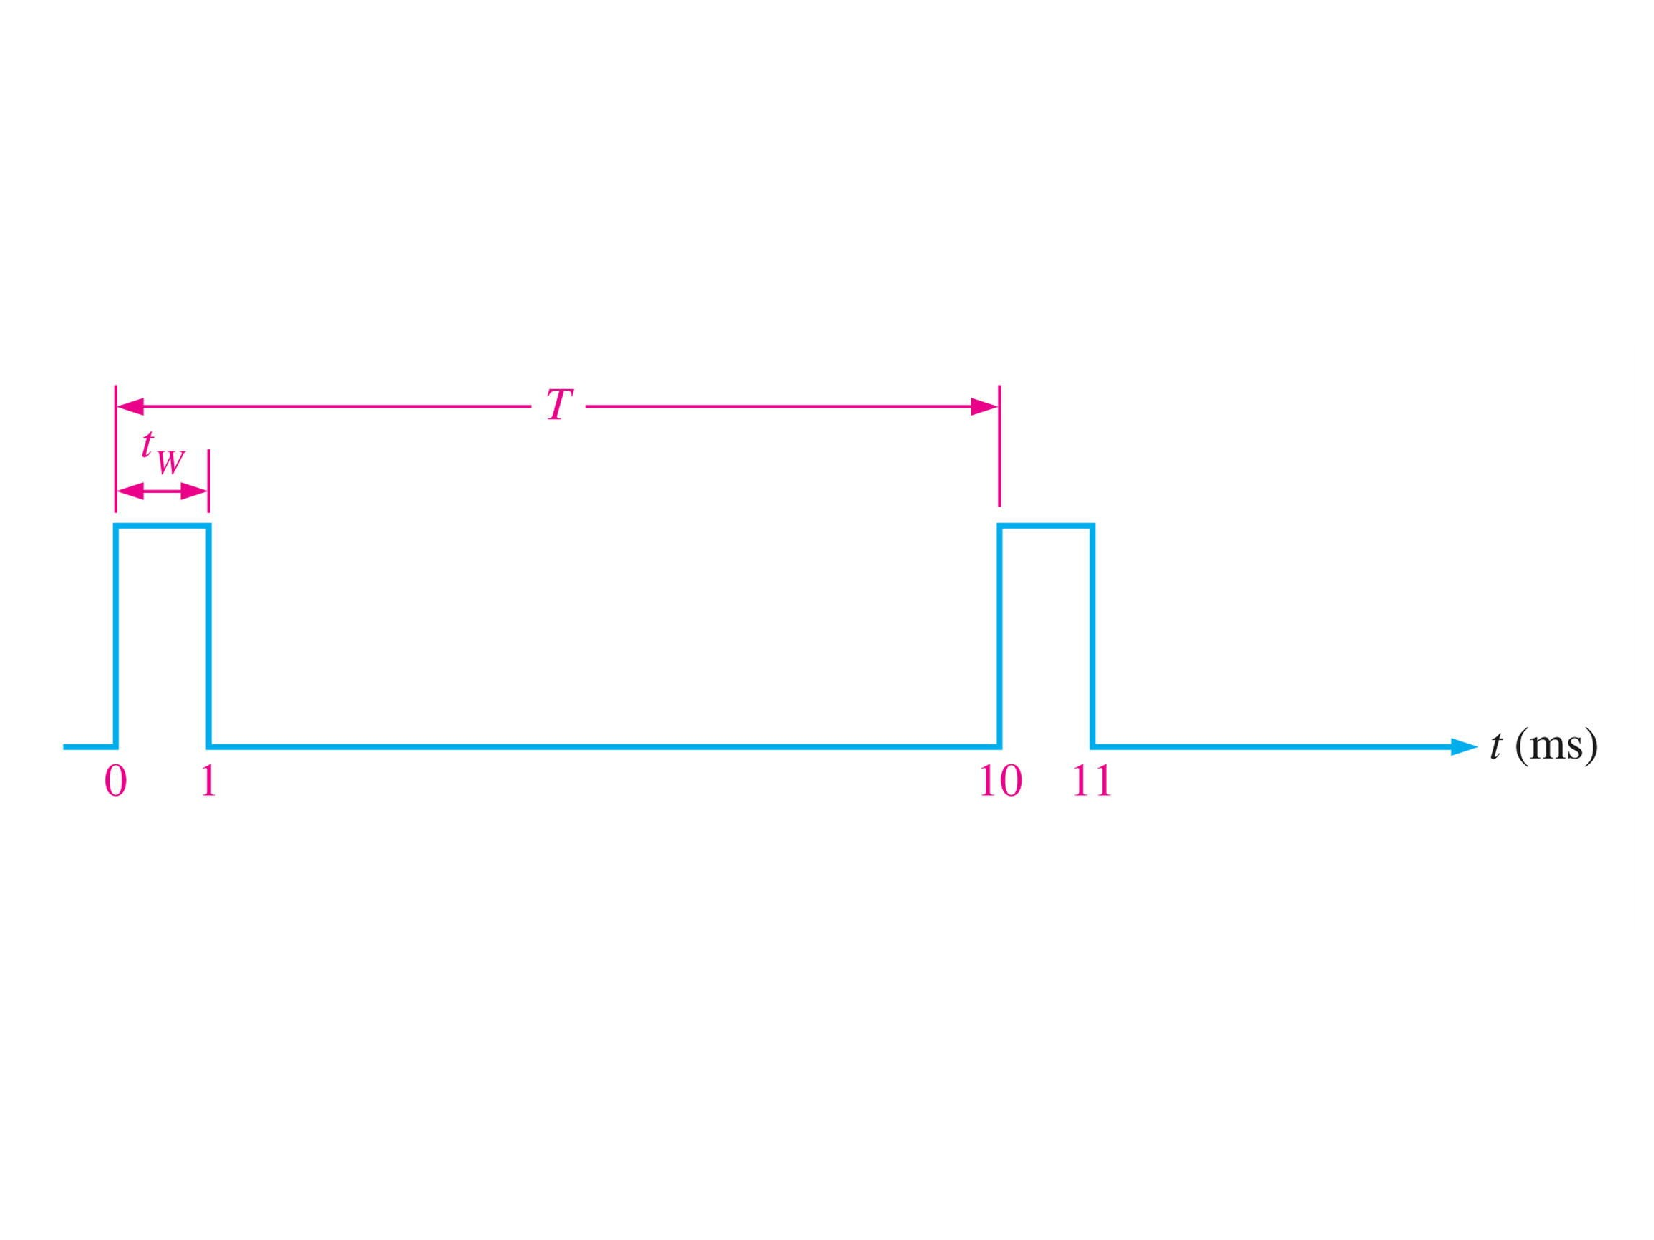
\includegraphics[width=0.8\textwidth,trim=0cm 4cm 0cm 4cm,clip=true]{digital3.pdf}
\caption{\label{fig:digital3} A periodic pulse demonstrating the concept of duty cycle. (Professor: do an example here and vary duty cycle).}
\textbf{What is the duty cycle in Fig. \ref{fig:digital3}?  What is the frequency?}
\end{figure}
\end{frame}

\begin{frame}{Logic Functions}
Logic function: mapping digital inputs to outputs.  A \textit{timing diagram} displays three digital inputs.
\begin{figure}
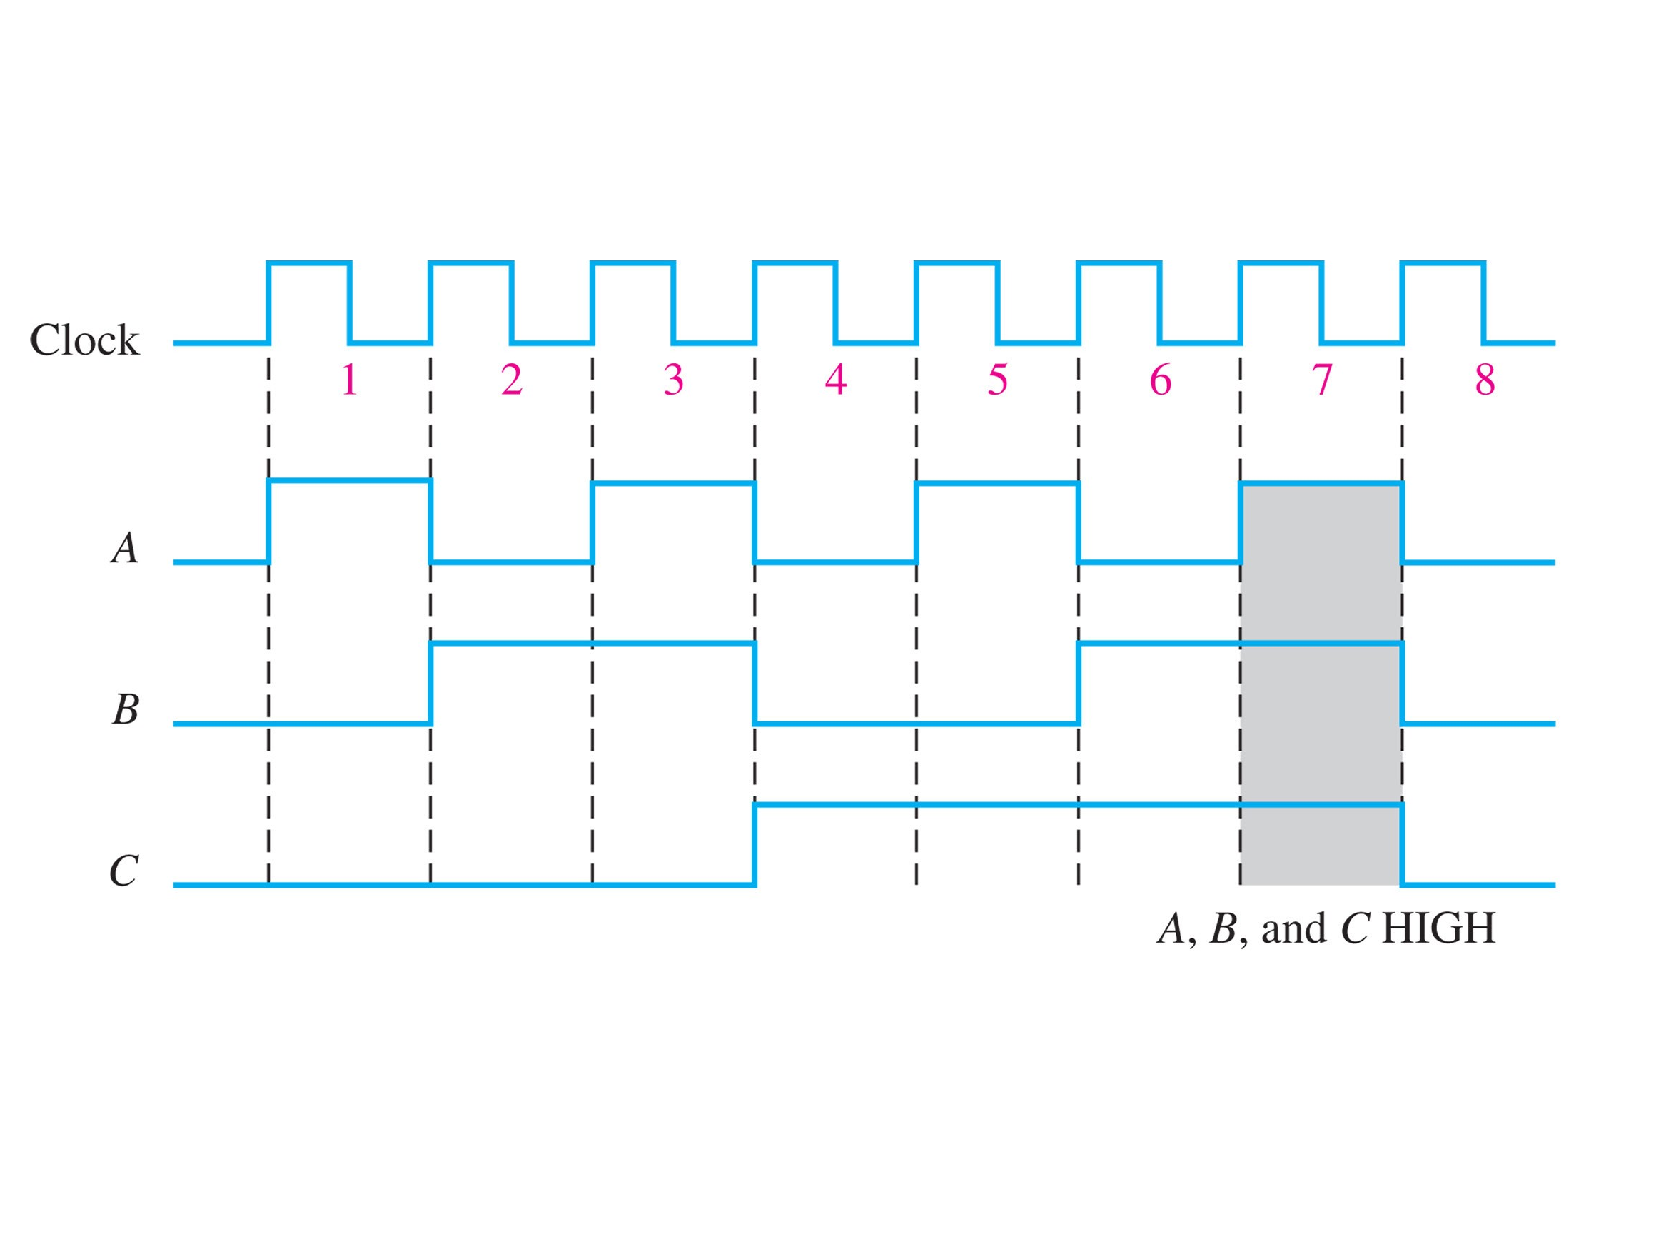
\includegraphics[width=0.8\textwidth,trim=0cm 4cm 0cm 4cm,clip=true]{digital4.pdf}
\caption{\label{fig:digital4} A logic function can be displayed as a timing diagram.  Add a forth input, labeled OUT.  Suppose OUT is only high when A, B, and C are all high.  Draw OUT versus time.}
\end{figure}
\end{frame}

\begin{frame}{Logic Functions}
Logic gates: fundamental blocks of logic functions.
\begin{figure}
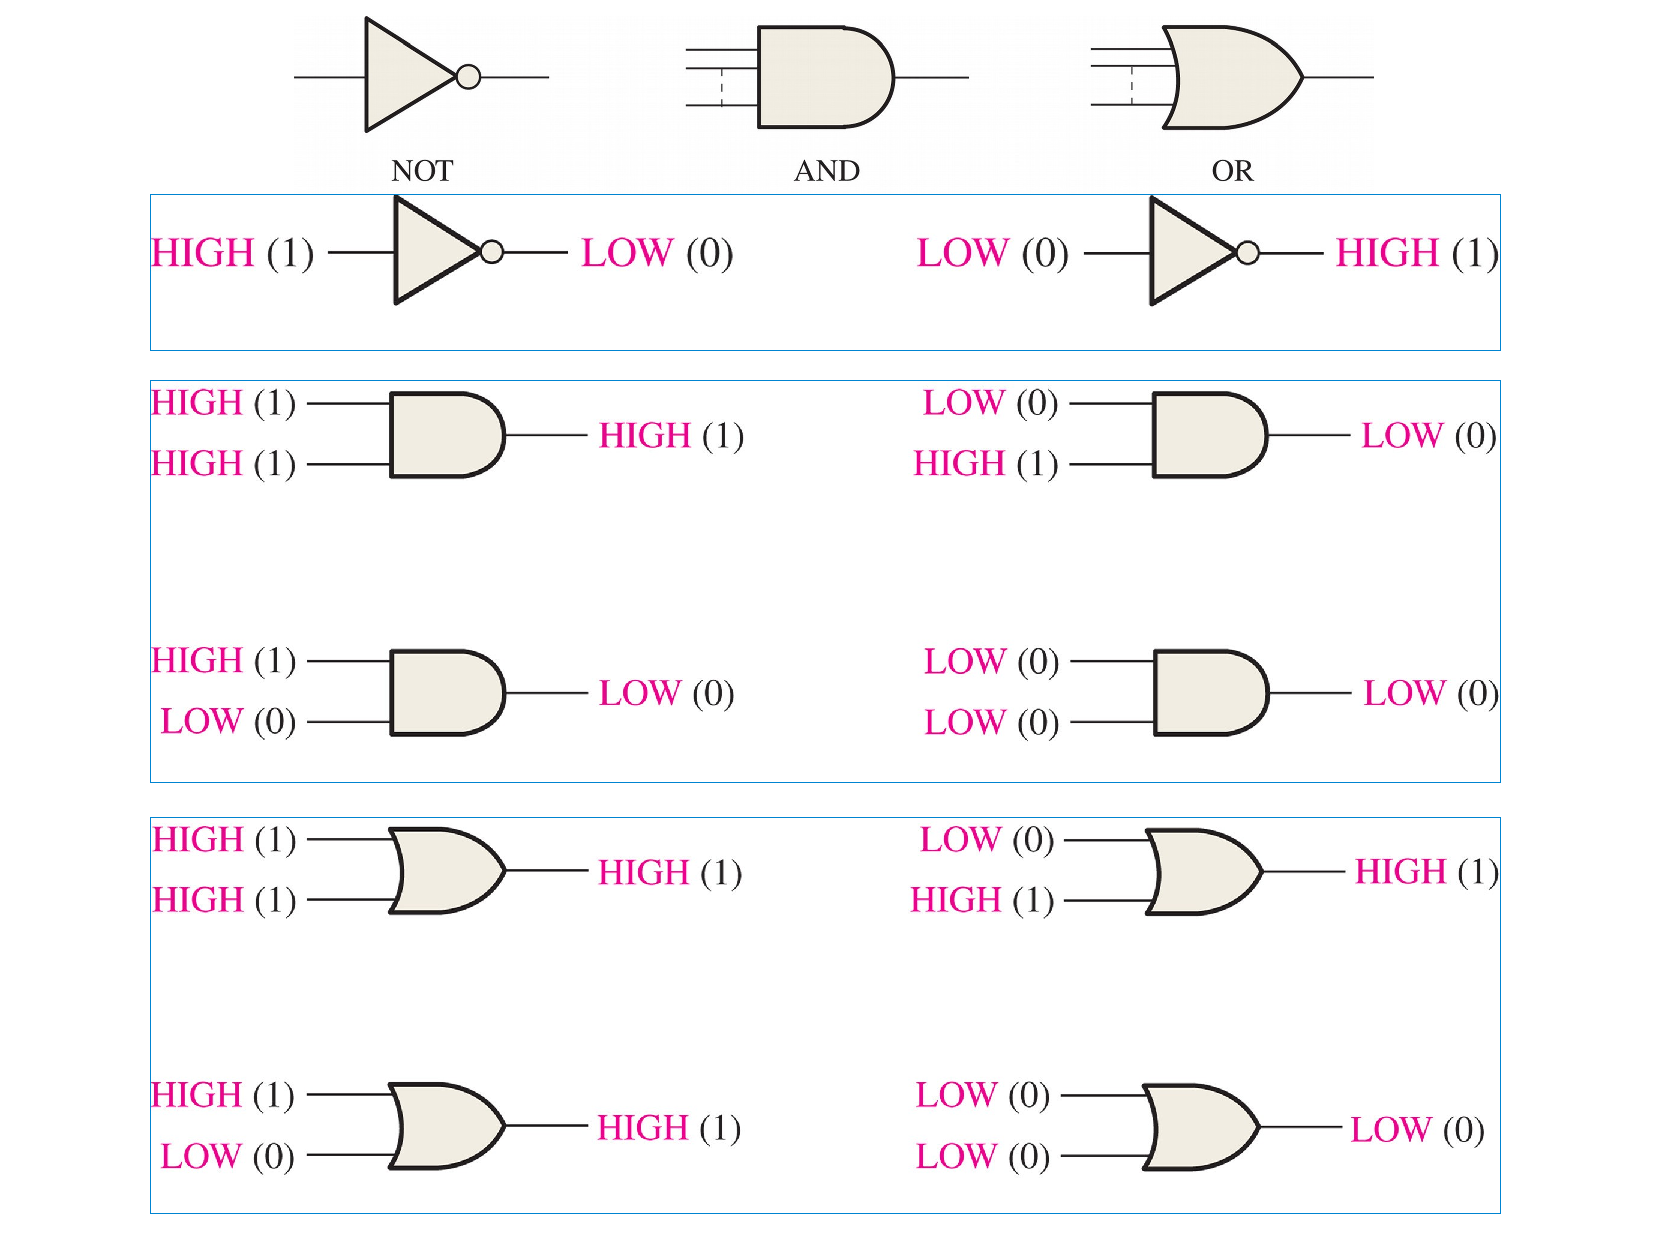
\includegraphics[width=0.7\textwidth]{gates1.pdf}
\caption{\label{fig:digital5} NOT, AND, and OR.  These gates are built from transistors, and have \textit{truth tables.}}
\end{figure}
\end{frame}

\begin{frame}{Logic Functions}
Logic gates: combinatoric functions are built from gates.
\begin{figure}
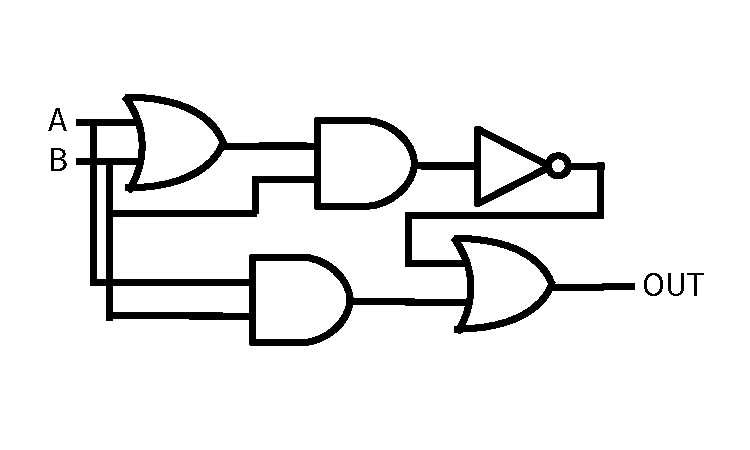
\includegraphics[width=0.7\textwidth]{operators2.pdf}
\caption{\label{fig:digital5_2} NOT, AND, and OR gates build up other functions.  What function is being described here?  What three states (values for A and B) would make OUT go high?}
\end{figure}
\end{frame}

\begin{frame}{Logic Functions}
Logic gates: combinatoric functions are built from gates.
\begin{figure}
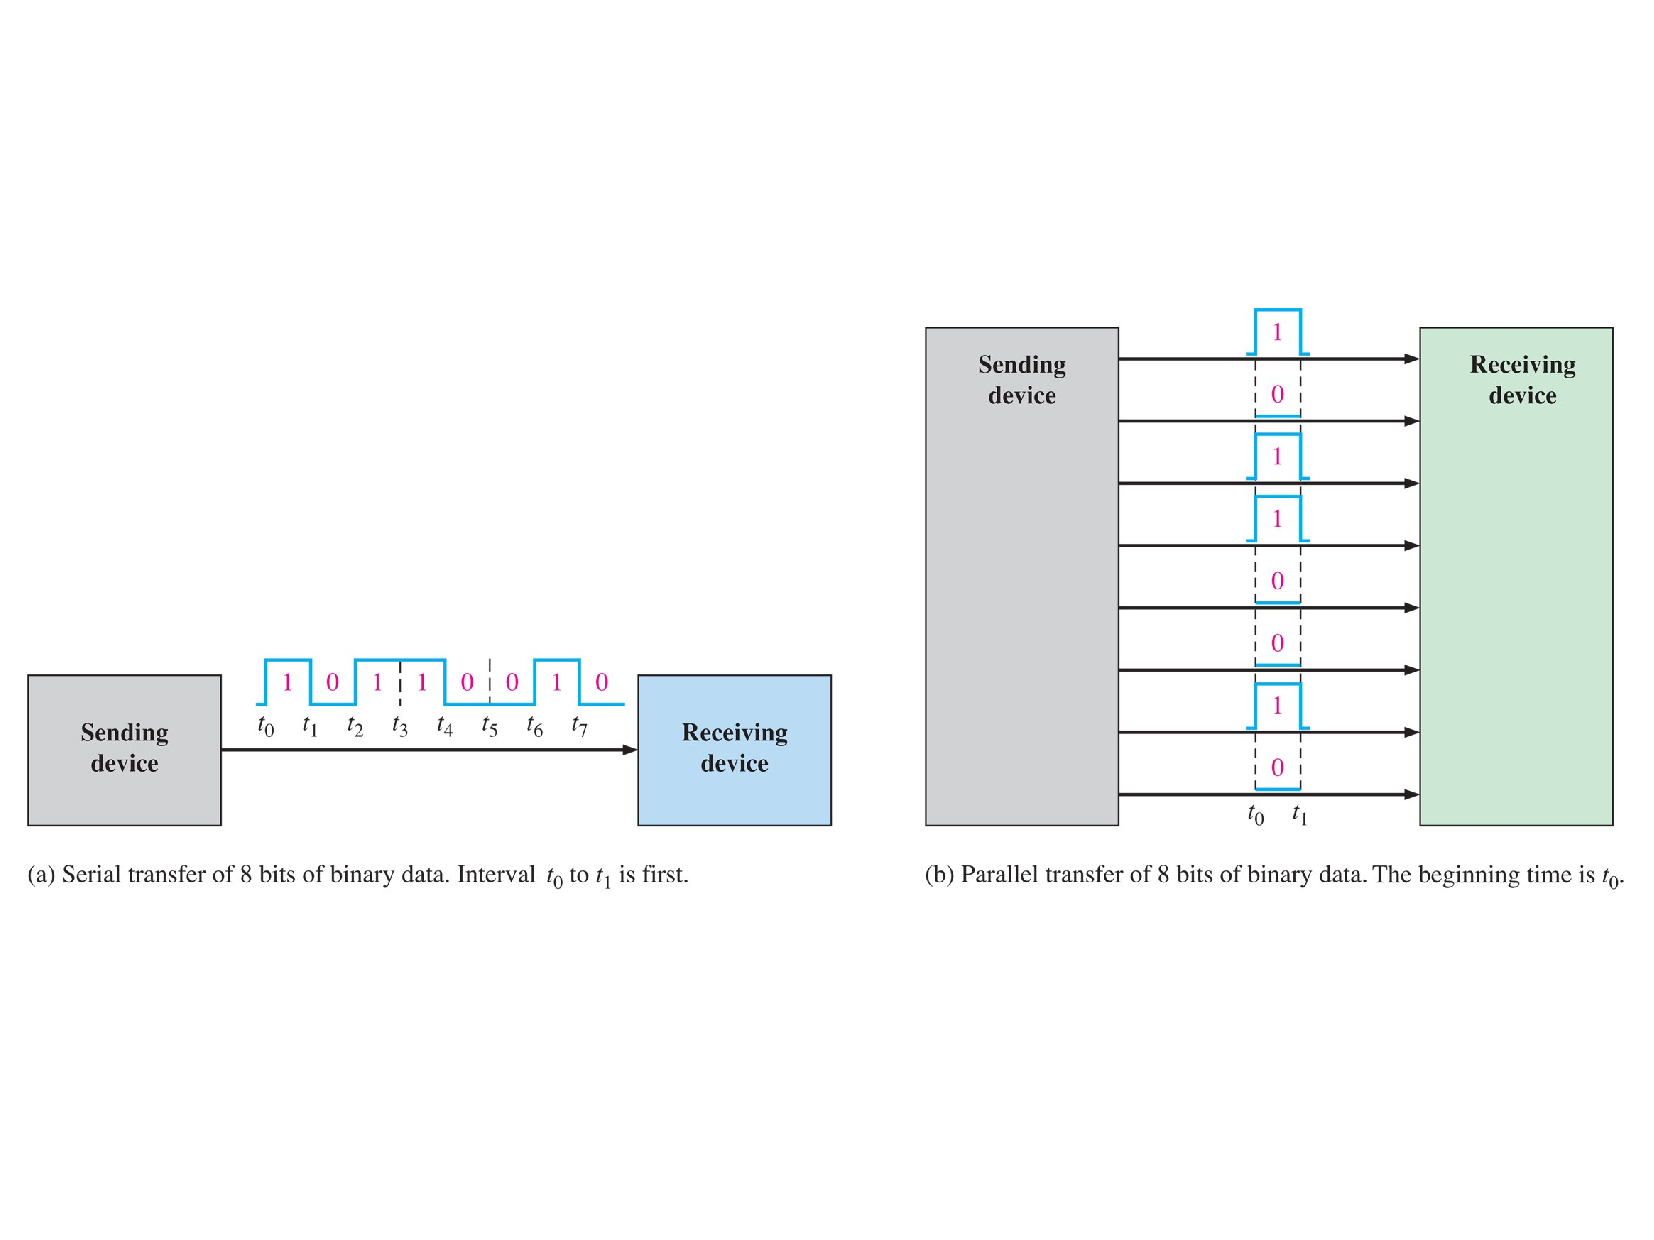
\includegraphics[width=0.8\textwidth,trim=0cm 4cm 0cm 4cm,clip=true]{digital5.pdf}
\caption{\label{fig:digital6} Combinatoric functions can exchange data in serial and parallel form.}
\end{figure}
\end{frame}

\section{PL versus IC}

\begin{frame}{PL versus IC}
\small
\begin{figure}
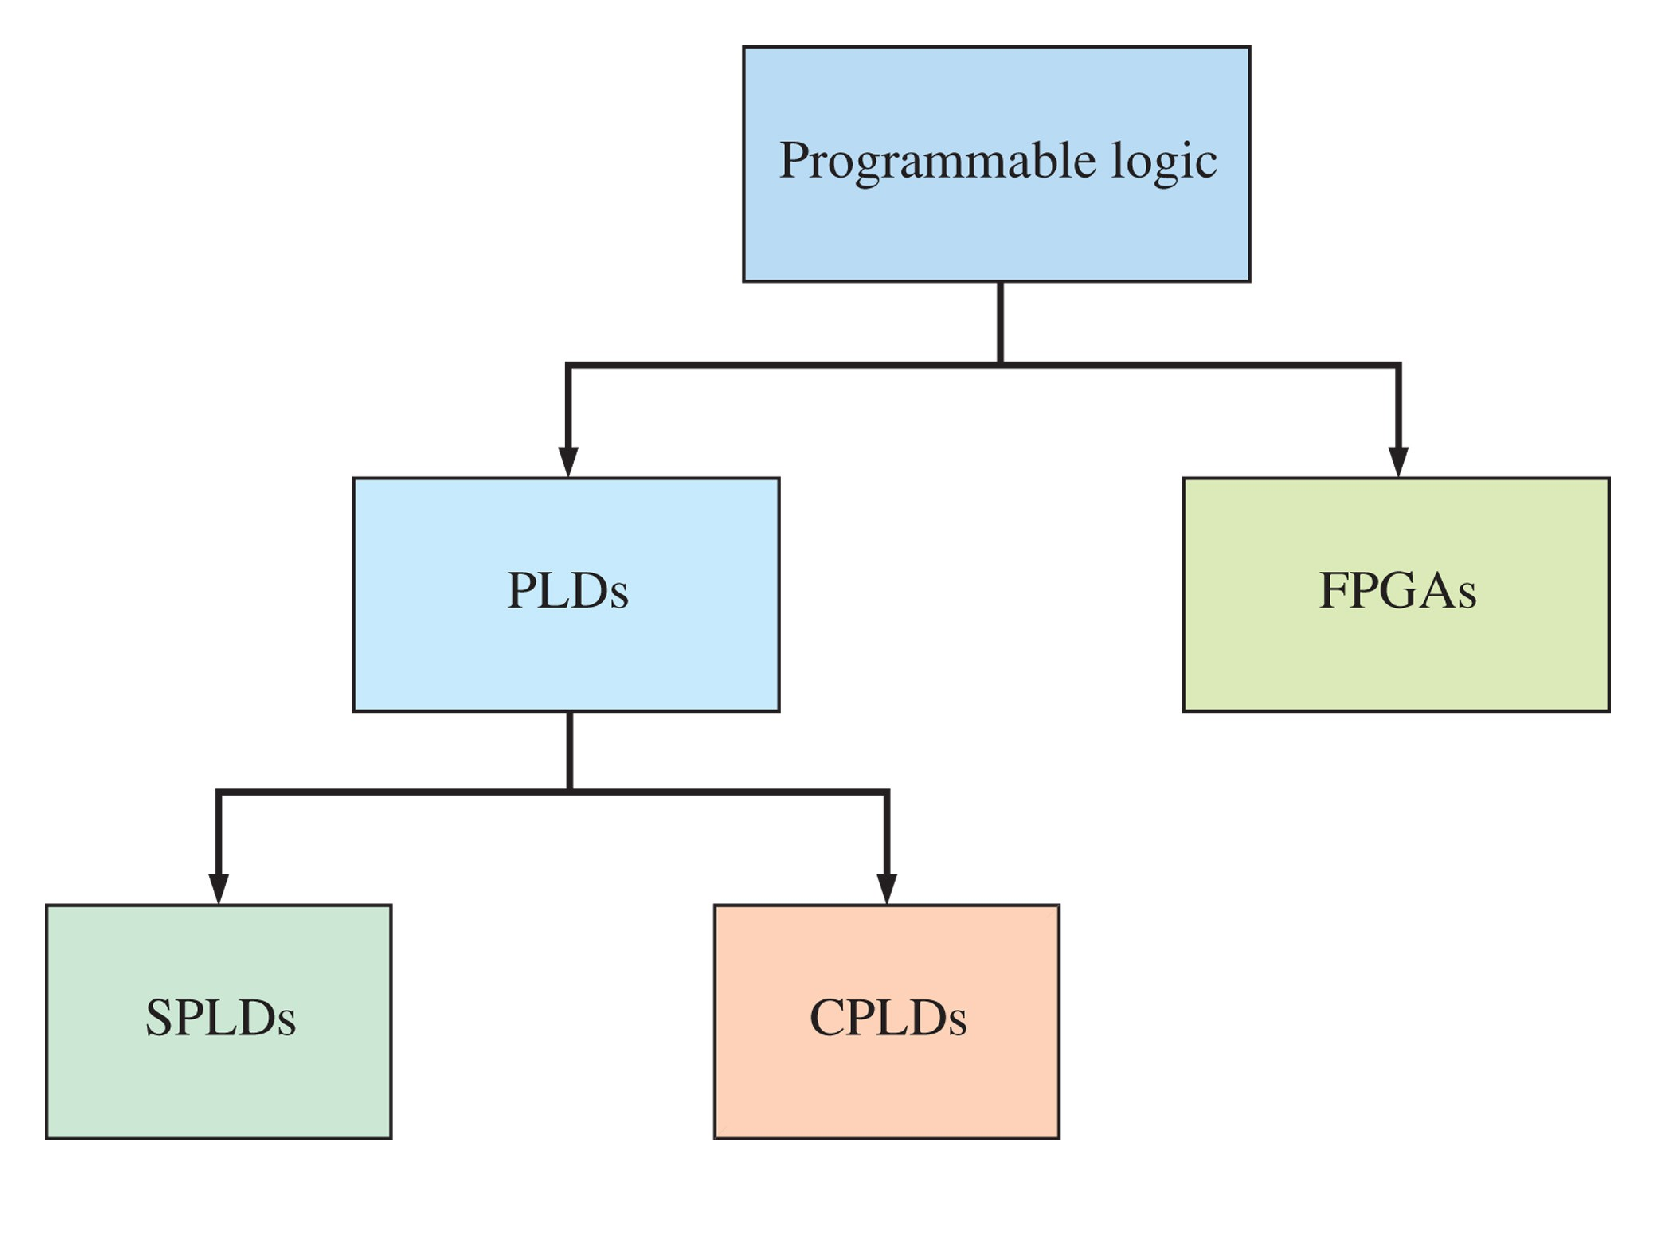
\includegraphics[width=0.75\textwidth]{PL.pdf}
\caption{\label{fig:PL1} Programmable logic falls into several categories. (a) Programmable logic devices (PLDs), simple and complex.  (b) Field Programmable Gate Arrays (FPGAs). }
\end{figure}
\end{frame}

\begin{frame}{PL versus IC}
\small
\begin{figure}
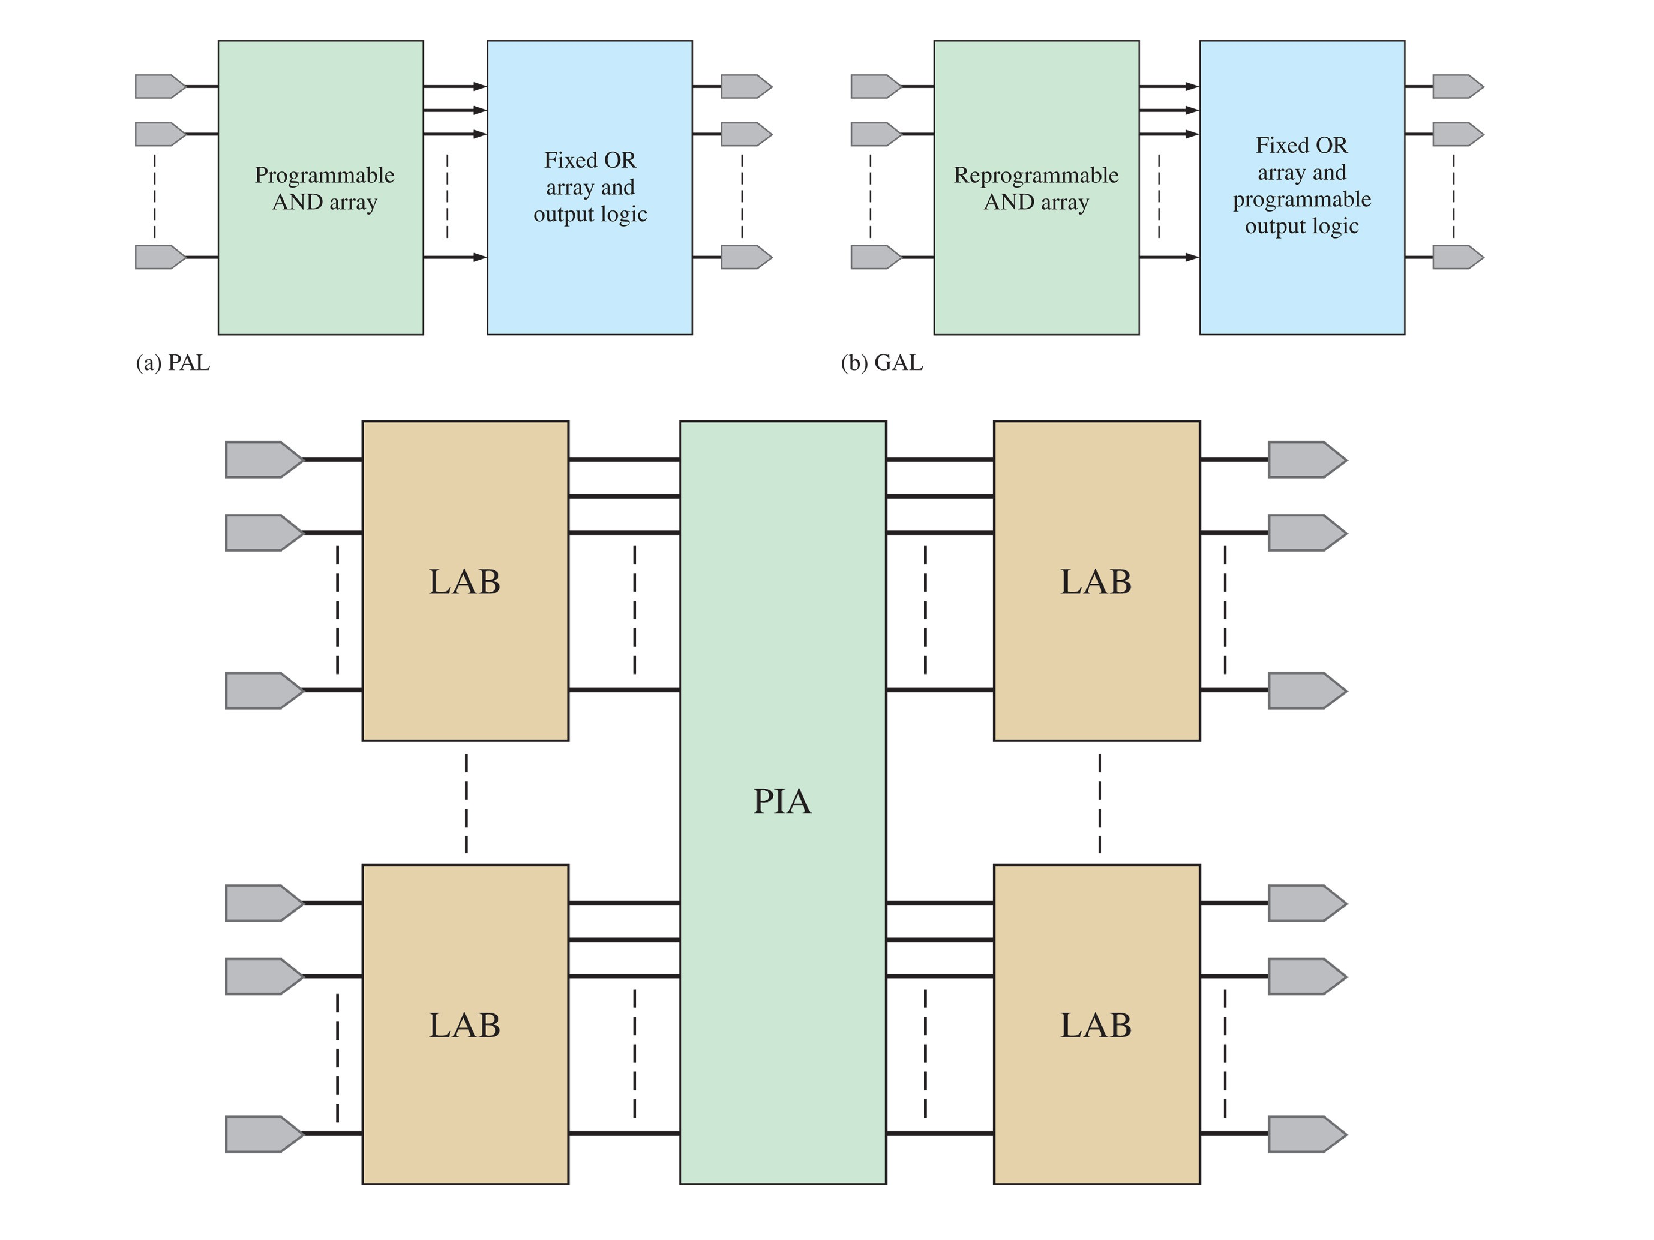
\includegraphics[width=0.75\textwidth]{PL2.pdf}
\caption{\label{fig:PL2} Programmable logic devices (PLDs), simple and complex.  Combinatoric logic functions can be built using these systems.}
\end{figure}
\end{frame}

\begin{frame}{PL versus IC}
\begin{figure}
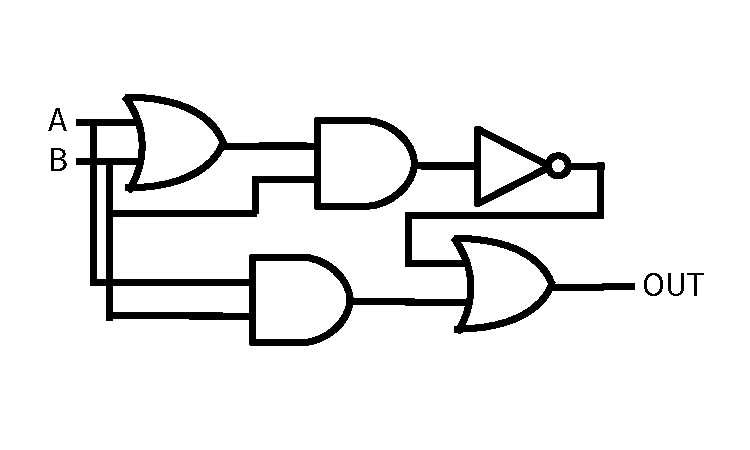
\includegraphics[width=0.7\textwidth]{operators2.pdf}
\caption{\label{fig:PL2a} This function reduces to $\bar{B} + AB$.}
\end{figure}
SPLD could be used to temporarily create this function.
\end{frame}

\begin{frame}{PL versus IC}
\small
\begin{figure}
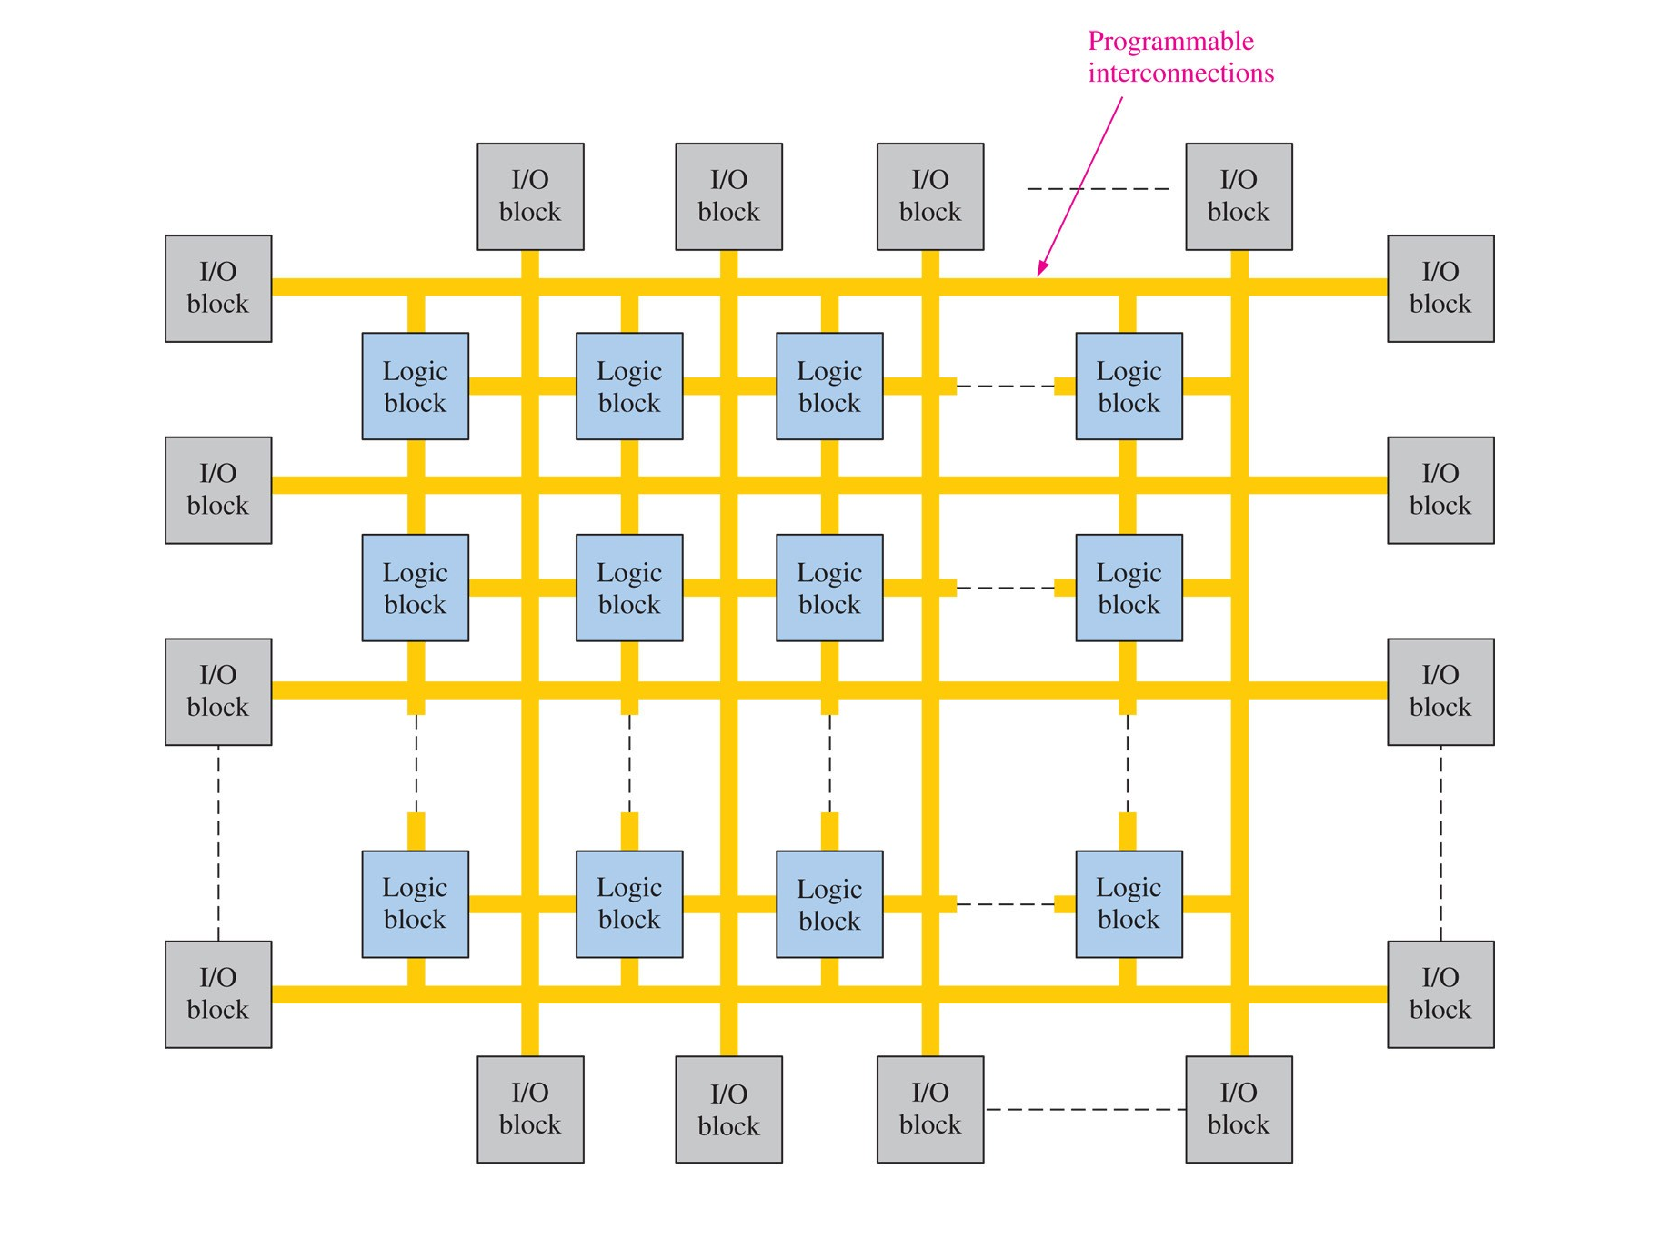
\includegraphics[width=0.75\textwidth]{PL3.pdf}
\caption{\label{fig:PL3} Field Programmable Gate Arrays (FPGAs) can be used to design vast, complex systems of logic functions.}
\end{figure}
\end{frame}

\begin{frame}{PL versus IC}
\small
\begin{figure}
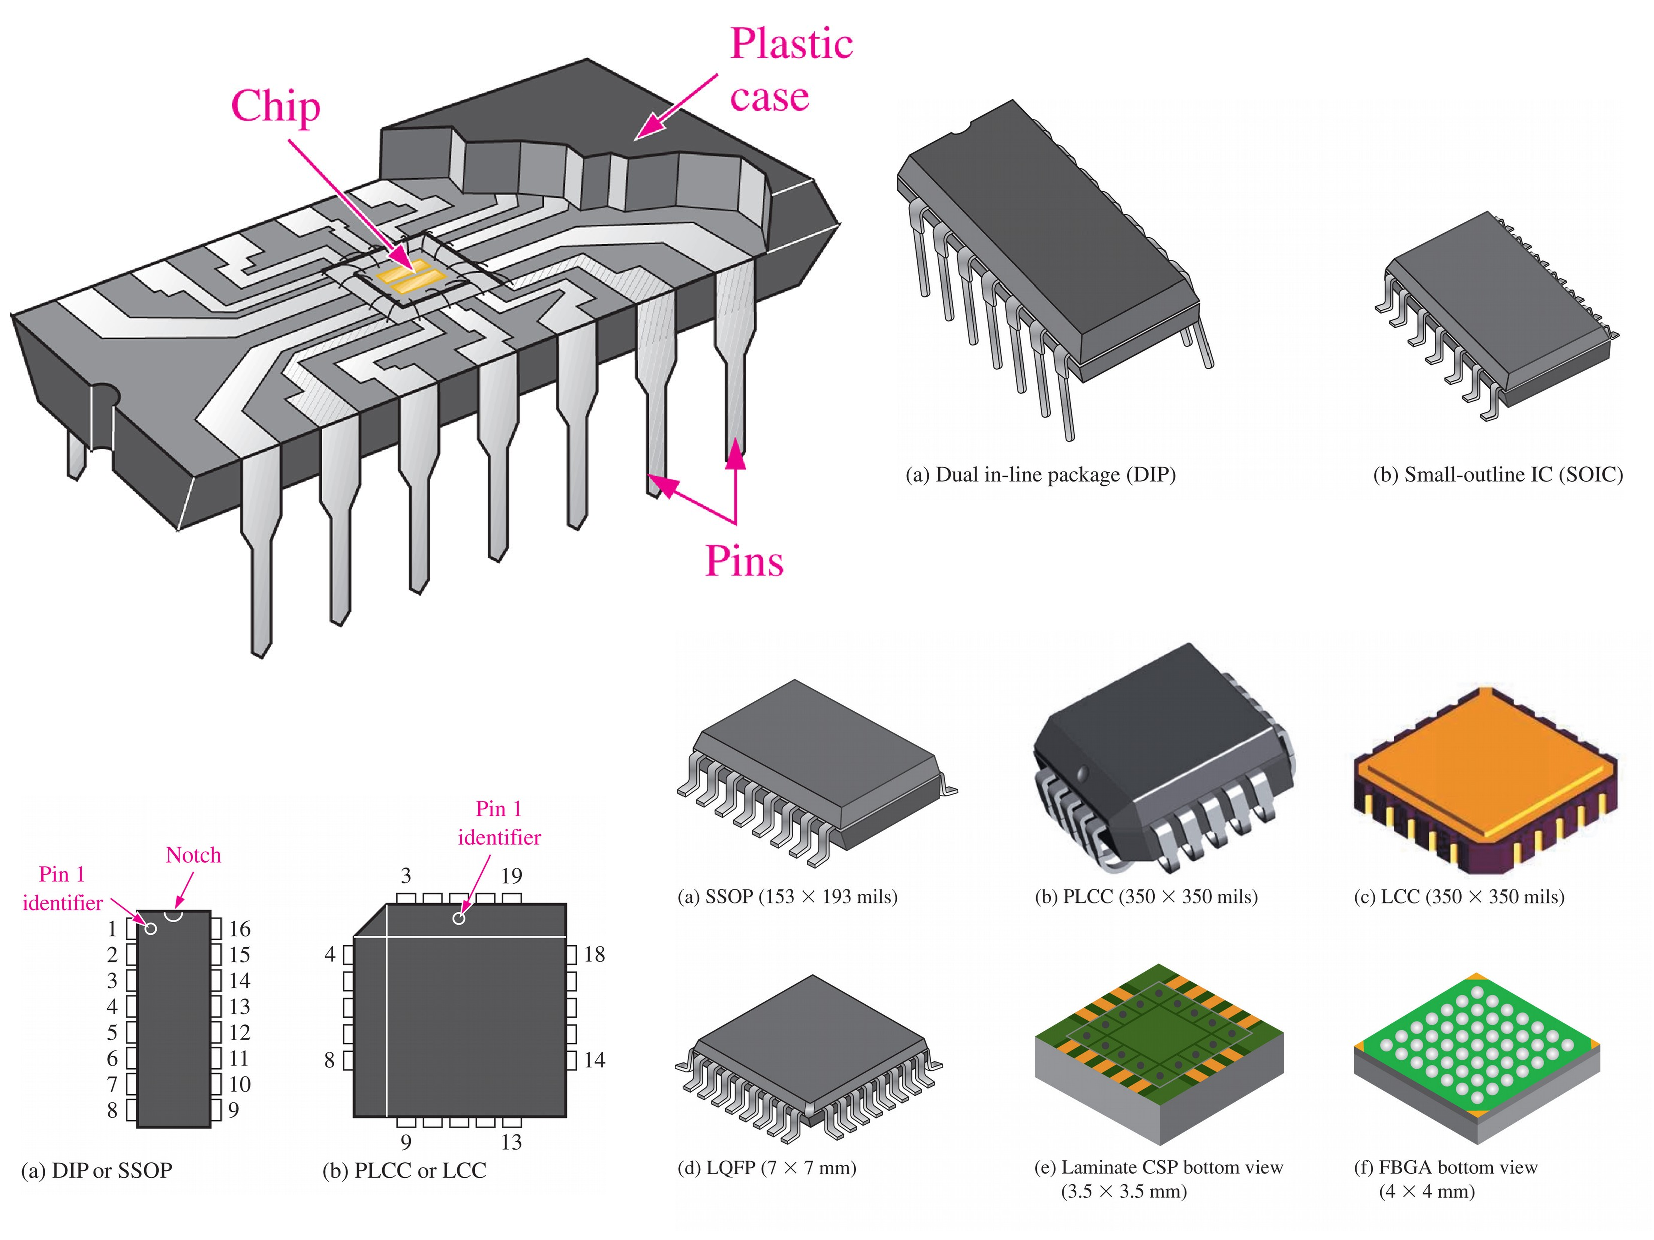
\includegraphics[width=0.75\textwidth]{PL4.pdf}
\caption{\label{fig:PL4} Various types of integrated circuits (ICs), that represent fixed combinatoric functions.  They come in through-hole and surface mount varieties.}
\end{figure}
\end{frame}

\section{Test Instruments}

\begin{frame}{Test Instruments}
\small
\begin{figure}
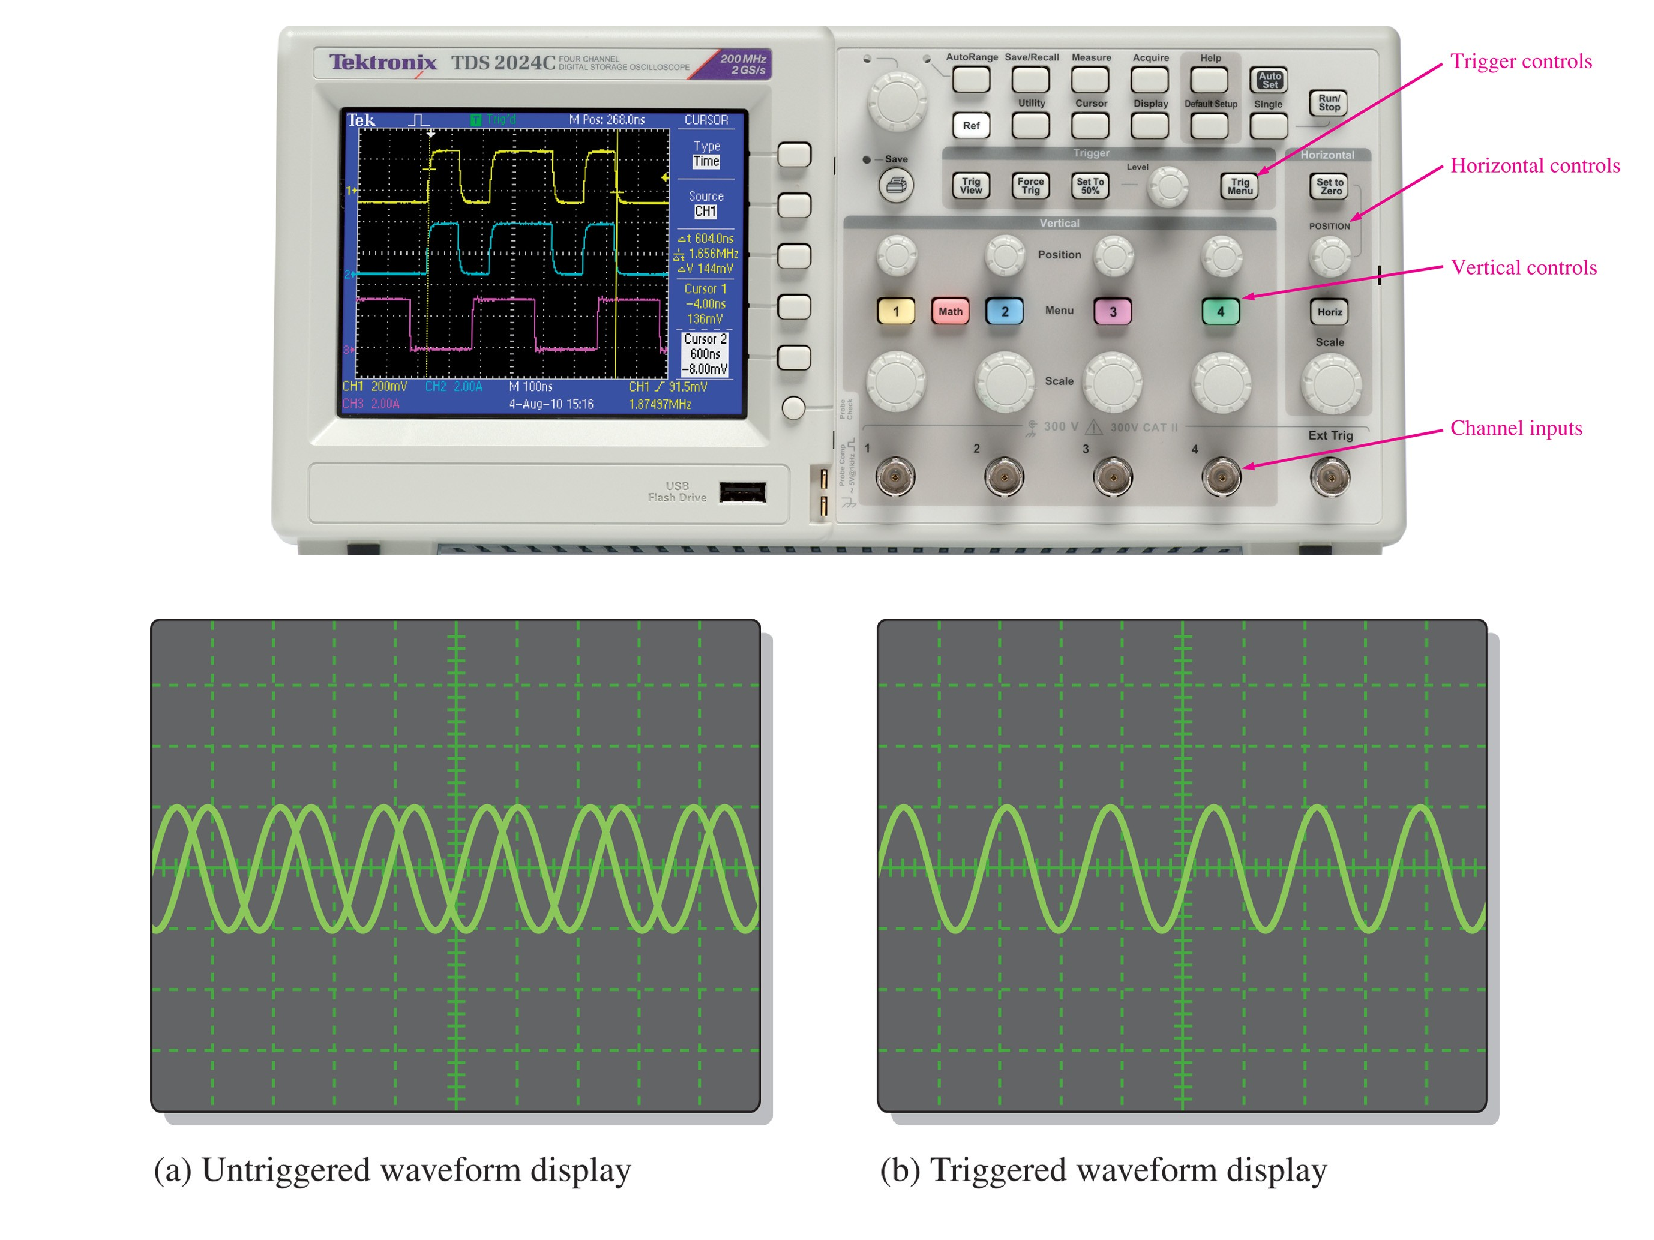
\includegraphics[width=0.75\textwidth]{scope1.pdf}
\caption{\label{fig:scope1} The oscilloscope plots digital and analog signals versus time.  The scope needs to \textit{trigger.}}
\end{figure}
\end{frame}

\begin{frame}{Test Instruments}
\small
\begin{figure}
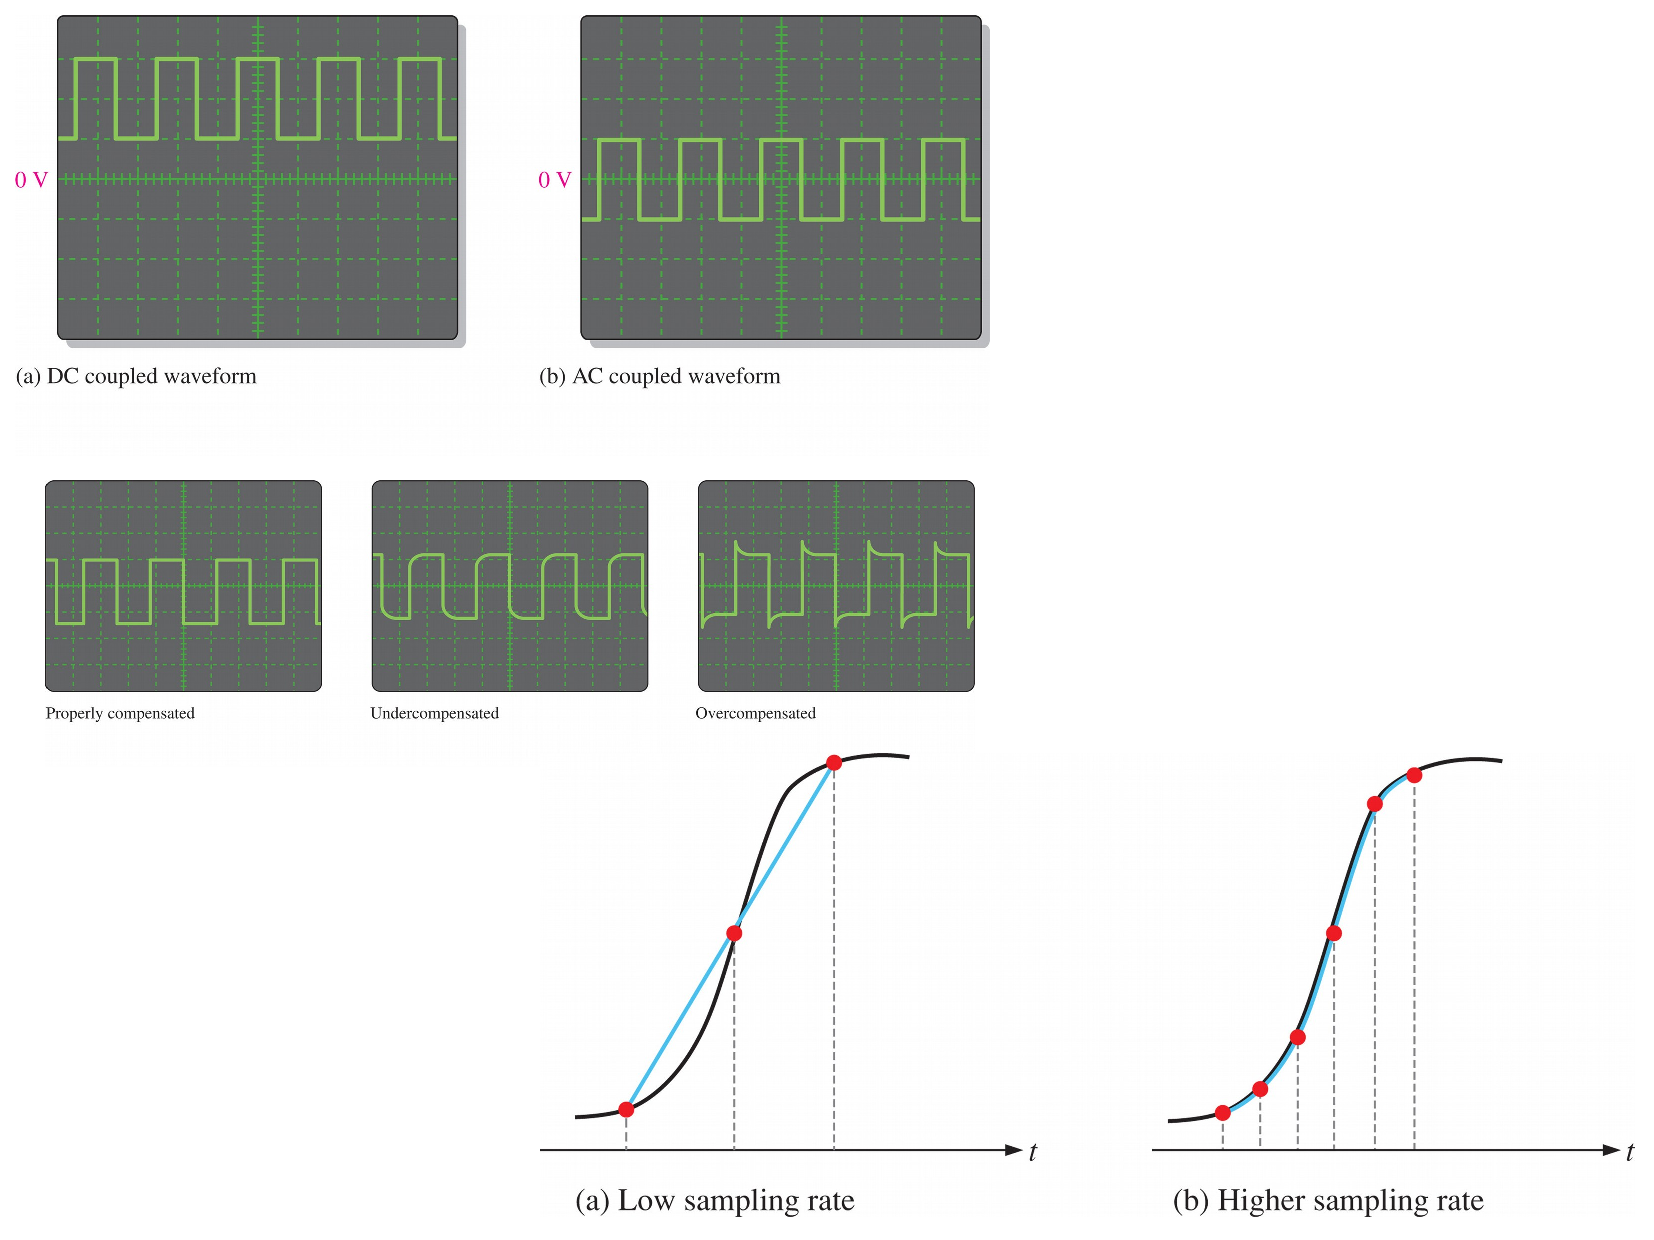
\includegraphics[width=0.75\textwidth]{scope2.pdf}
\caption{\label{fig:scope2} The scope needs to \textit{sample} at a high enough sampling rate to compensate for frequency of data.  There's also the issue of AC versus DC coupling.  (Professor: do some examples here).}
\end{figure}
\end{frame}

\begin{frame}{Test Instruments}
\begin{figure}
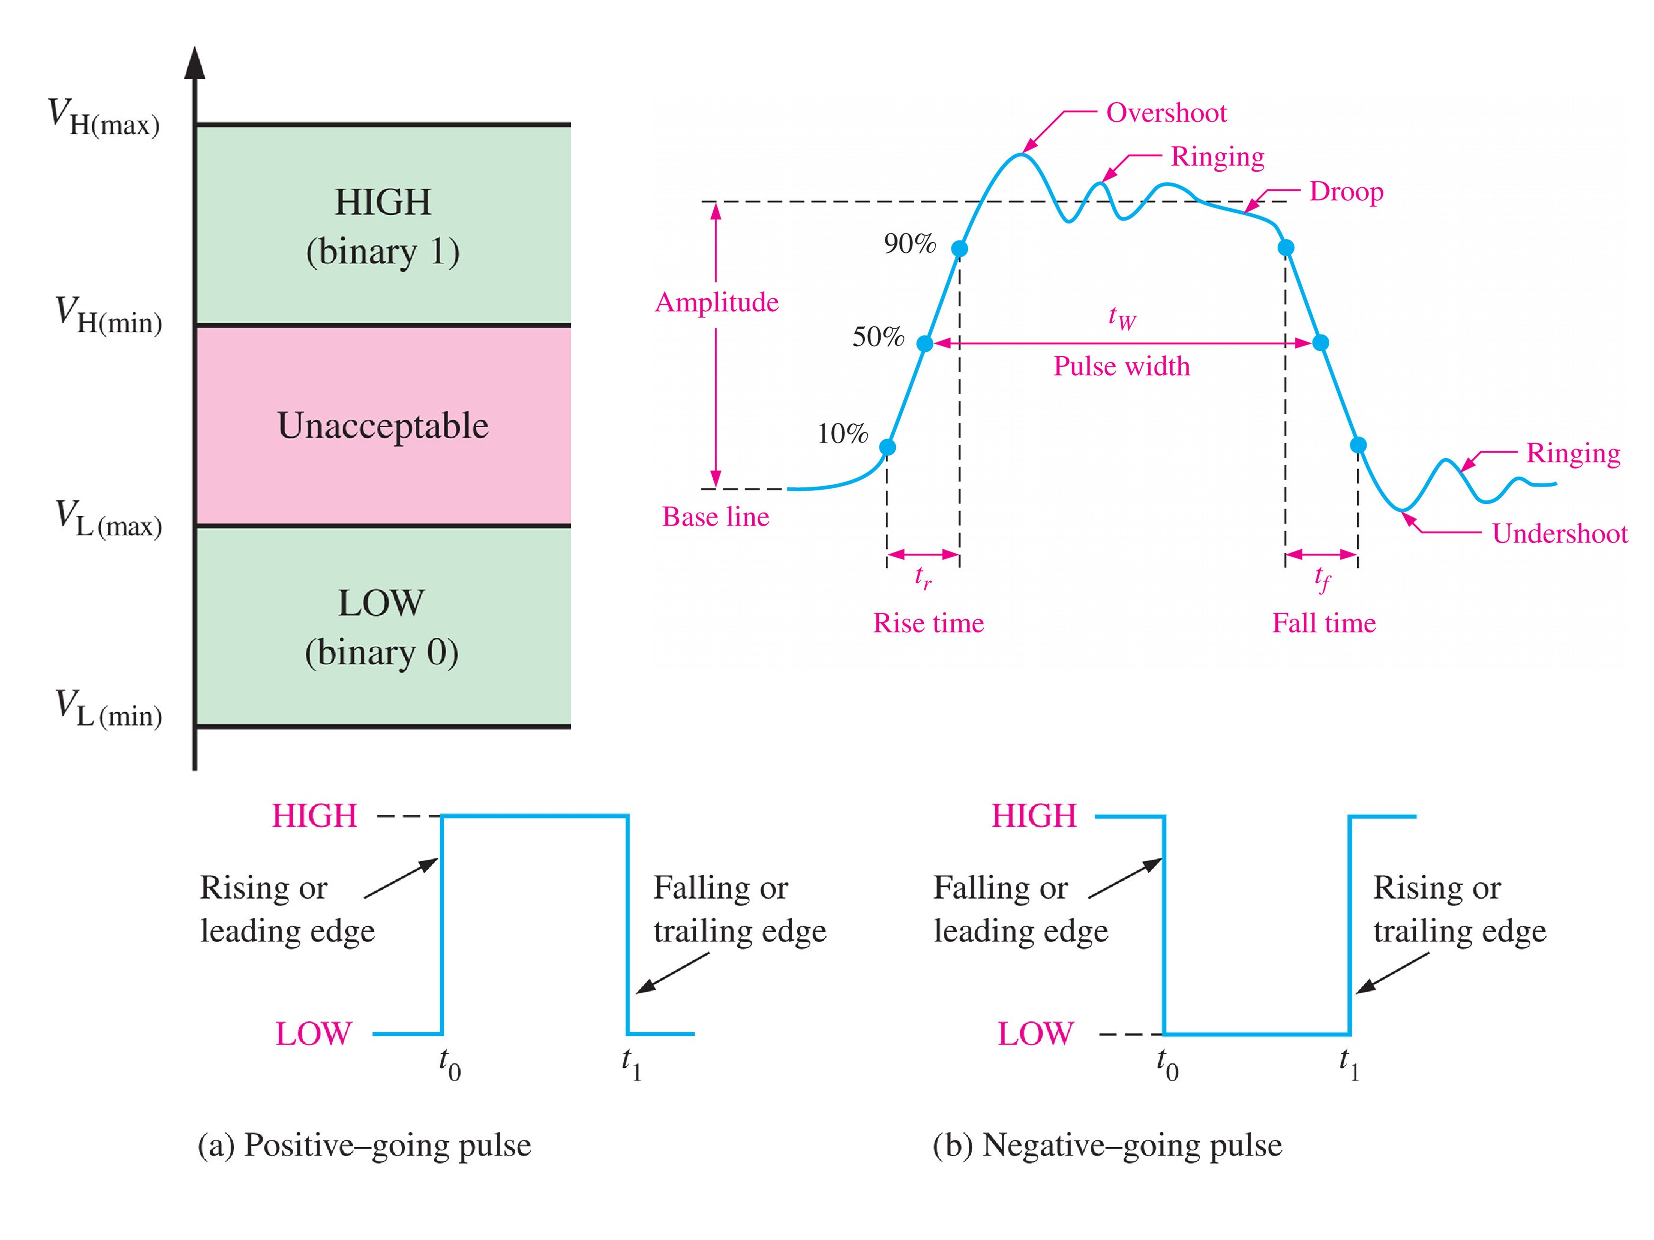
\includegraphics[width=0.75\textwidth]{digital1.pdf}
\caption{\label{fig:digital1_2} With this issue, we begin our laboratory activity.}
\end{figure}
\end{frame}

\section{Conclusion}

\begin{frame}{Summary}
\begin{enumerate}
\item Logic functions
\begin{itemize}
\item Basic gate ideas
\item Combinatorial logic functions
\item Serial and parallel
\end{itemize}
\item Programmable logic (PL) vs. fixed integrated circuits (ICs)
\item Test instruments
\begin{itemize}
\item Oscilloscope
\item Signal generator
\item Digital voltmeter and DC power supply
\end{itemize}
\end{enumerate}
\end{frame}

\end{document}
